\documentclass[twoside]{book}

% Packages required by doxygen
\usepackage{calc}
\usepackage{doxygen}
\usepackage{graphicx}
\usepackage[utf8]{inputenc}
\usepackage{makeidx}
\usepackage{multicol}
\usepackage{multirow}
\usepackage{textcomp}
\usepackage[table]{xcolor}

% Font selection
\usepackage[T1]{fontenc}
\usepackage{mathptmx}
\usepackage[scaled=.90]{helvet}
\usepackage{courier}
\usepackage{amssymb}
\usepackage{sectsty}
\renewcommand{\familydefault}{\sfdefault}
\allsectionsfont{%
  \fontseries{bc}\selectfont%
  \color{darkgray}%
}
\renewcommand{\DoxyLabelFont}{%
  \fontseries{bc}\selectfont%
  \color{darkgray}%
}

% Page & text layout
\usepackage{geometry}
\geometry{%
  a4paper,%
  top=2.5cm,%
  bottom=2.5cm,%
  left=2.5cm,%
  right=2.5cm%
}
\tolerance=750
\hfuzz=15pt
\hbadness=750
\setlength{\emergencystretch}{15pt}
\setlength{\parindent}{0cm}
\setlength{\parskip}{0.2cm}
\makeatletter
\renewcommand{\paragraph}{%
  \@startsection{paragraph}{4}{0ex}{-1.0ex}{1.0ex}{%
    \normalfont\normalsize\bfseries\SS@parafont%
  }%
}
\renewcommand{\subparagraph}{%
  \@startsection{subparagraph}{5}{0ex}{-1.0ex}{1.0ex}{%
    \normalfont\normalsize\bfseries\SS@subparafont%
  }%
}
\makeatother

% Headers & footers
\usepackage{fancyhdr}
\pagestyle{fancyplain}
\fancyhead[LE]{\fancyplain{}{\bfseries\thepage}}
\fancyhead[CE]{\fancyplain{}{}}
\fancyhead[RE]{\fancyplain{}{\bfseries\leftmark}}
\fancyhead[LO]{\fancyplain{}{\bfseries\rightmark}}
\fancyhead[CO]{\fancyplain{}{}}
\fancyhead[RO]{\fancyplain{}{\bfseries\thepage}}
\fancyfoot[LE]{\fancyplain{}{}}
\fancyfoot[CE]{\fancyplain{}{}}
\fancyfoot[RE]{\fancyplain{}{\bfseries\scriptsize Generated on Fri Apr 25 2014 22\-:24\-:41 for Glossygloss by Doxygen }}
\fancyfoot[LO]{\fancyplain{}{\bfseries\scriptsize Generated on Fri Apr 25 2014 22\-:24\-:41 for Glossygloss by Doxygen }}
\fancyfoot[CO]{\fancyplain{}{}}
\fancyfoot[RO]{\fancyplain{}{}}
\renewcommand{\footrulewidth}{0.4pt}
\renewcommand{\chaptermark}[1]{%
  \markboth{#1}{}%
}
\renewcommand{\sectionmark}[1]{%
  \markright{\thesection\ #1}%
}

% Indices & bibliography
\usepackage{natbib}
\usepackage[titles]{tocloft}
\setcounter{tocdepth}{3}
\setcounter{secnumdepth}{5}
\makeindex

% Hyperlinks (required, but should be loaded last)
\usepackage{ifpdf}
\ifpdf
  \usepackage[pdftex,pagebackref=true]{hyperref}
\else
  \usepackage[ps2pdf,pagebackref=true]{hyperref}
\fi
\hypersetup{%
  colorlinks=true,%
  linkcolor=blue,%
  citecolor=blue,%
  unicode%
}

% Custom commands
\newcommand{\clearemptydoublepage}{%
  \newpage{\pagestyle{empty}\cleardoublepage}%
}


%===== C O N T E N T S =====

\begin{document}

% Titlepage & ToC
\hypersetup{pageanchor=false}
\pagenumbering{roman}
\begin{titlepage}
\vspace*{7cm}
\begin{center}%
{\Large Glossygloss \\[1ex]\large 0.\-2 }\\
\vspace*{1cm}
{\large Generated by Doxygen 1.8.6}\\
\vspace*{0.5cm}
{\small Fri Apr 25 2014 22:24:41}\\
\end{center}
\end{titlepage}
\clearemptydoublepage
\tableofcontents
\clearemptydoublepage
\pagenumbering{arabic}
\hypersetup{pageanchor=true}

%--- Begin generated contents ---
\chapter{Main Page}
\label{index}\hypertarget{index}{}Glossygloss is set of classes to use several data structures, C++ containers. More might come soon.

\subsubsection*{Documentation}

All documented things are \href{http://blasterbug.github.io/glossygloss/}{\tt here}.

A P\-D\-F file {\itshape refman.\-pdf} is also available for offline doc.

You can generate the doc using \href{http://www.stack.nl/~dimitri/doxygen/}{\tt doxygen} and the config file {\itshape doxygen\-\_\-config}

Usefull links \-:
\begin{DoxyItemize}
\item \href{http://en.wikibooks.org/wiki/C%2B%2B_Programming}{\tt C++ programming on wikibooks}
\item what else ?
\end{DoxyItemize}

\subsubsection*{Compilation}

Here is a sort intance showing how to compile and 'use' \hyperlink{hashtable_8hpp}{hashtable.\-hpp}. It works as well for others files.

We use C++11, so to compile using our classes\-:

\$ g++ -\/std=c++0x -\/\-Wall -\/pedantic -\/o sample\-\_\-hashtable.\-bin \hyperlink{sample__hashtable_8cpp}{sample\-\_\-hashtable.\-cpp}

\subsubsection*{Testing and usage}

Once you compiled \hyperlink{sample__hashtable_8cpp}{sample\-\_\-hashtable.\-cpp}, you can run the code using, assuming you are using an U\-N\-I\-X system.

\$ chmod +x sample\-\_\-hashtable.\-bin

First give execution permission to the compiled code.

\$ ./sample\-\_\-hashtable.bin lorem quod 50

And then, run the program. Words in the first file (lorem) will be maped to the words in quod. The last argument stands for the words number you want to put in the hashtable.

\subsubsection*{Copyright}

This source code is protected by the French intellectual property law.

This program is free software; you can redistribute it and/or modify it under the terms of the G\-N\-U General Public License as published by the Free Software Foundation; version 2 of the License.

This program is distributed in the hope that it will be useful, but W\-I\-T\-H\-O\-U\-T A\-N\-Y W\-A\-R\-R\-A\-N\-T\-Y; without even the implied warranty of M\-E\-R\-C\-H\-A\-N\-T\-A\-B\-I\-L\-I\-T\-Y or F\-I\-T\-N\-E\-S\-S F\-O\-R A P\-A\-R\-T\-I\-C\-U\-L\-A\-R P\-U\-R\-P\-O\-S\-E. See the G\-N\-U General Public License for more details. 
\chapter{Todo List}
\label{todo}
\hypertarget{todo}{}

\begin{DoxyRefList}
\item[\label{todo__todo000001}%
\hypertarget{todo__todo000001}{}%
File \hyperlink{hashtable_8hpp}{hashtable.hpp} ]\-: removing the last element of a alveoles chain makes trouble (seg fault) 
\end{DoxyRefList}
\chapter{Hierarchical Index}
\section{Class Hierarchy}
This inheritance list is sorted roughly, but not completely, alphabetically\-:\begin{DoxyCompactList}
\item \contentsline{section}{Alveole}{\pageref{class_alveole}}{}
\item exception\begin{DoxyCompactList}
\item \contentsline{section}{Hash\-Exception}{\pageref{class_hash_exception}}{}
\end{DoxyCompactList}
\item \contentsline{section}{Knot}{\pageref{class_knot}}{}
\item \contentsline{section}{Knot$<$ T $>$}{\pageref{class_knot}}{}
\item \contentsline{section}{Tree}{\pageref{class_tree}}{}
\end{DoxyCompactList}

\chapter{Class Index}
\section{Class List}
Here are the classes, structs, unions and interfaces with brief descriptions\-:\begin{DoxyCompactList}
\item\contentsline{section}{\hyperlink{class_alveole}{Alveole$<$ K, V $>$} \\*Class to define \hyperlink{class_hashtable}{Hashtable} alveoles }{\pageref{class_alveole}}{}
\item\contentsline{section}{\hyperlink{class_dictionnaire}{Dictionnaire} }{\pageref{class_dictionnaire}}{}
\item\contentsline{section}{\hyperlink{class_hashtable}{Hashtable$<$ K, V $>$} \\*Maps a key to a value }{\pageref{class_hashtable}}{}
\item\contentsline{section}{\hyperlink{class_hashtable_exception}{Hashtable\-Exception} \\*Exception class to manage \hyperlink{class_hashtable}{Hashtable} errors }{\pageref{class_hashtable_exception}}{}
\item\contentsline{section}{\hyperlink{class_node}{Node$<$ T $>$} \\*Defines tree nodes }{\pageref{class_node}}{}
\item\contentsline{section}{\hyperlink{class_tree}{Tree$<$ T $>$} \\*\hyperlink{class_tree}{Tree} is a recursive structure using nodes }{\pageref{class_tree}}{}
\item\contentsline{section}{\hyperlink{class_tree_exception}{Tree\-Exception} \\*Exception class for trees }{\pageref{class_tree_exception}}{}
\item\contentsline{section}{\hyperlink{class_tree_string}{Tree\-String} \\*\hyperlink{class_tree}{Tree} is a recursive structure using nodes }{\pageref{class_tree_string}}{}
\item\contentsline{section}{\hyperlink{class_tree_string_exception}{Tree\-String\-Exception} \\*Exception class for trees }{\pageref{class_tree_string_exception}}{}
\end{DoxyCompactList}

\chapter{File Index}
\section{File List}
Here is a list of all files with brief descriptions\-:\begin{DoxyCompactList}
\item\contentsline{section}{\hyperlink{_hash_exception_8hpp}{Hash\-Exception.\-hpp} }{\pageref{_hash_exception_8hpp}}{}
\item\contentsline{section}{\hyperlink{_hash_table_8hpp}{Hash\-Table.\-hpp} }{\pageref{_hash_table_8hpp}}{}
\item\contentsline{section}{\hyperlink{tree_8hpp}{tree.\-hpp} }{\pageref{tree_8hpp}}{}
\end{DoxyCompactList}

\chapter{Class Documentation}
\hypertarget{class_alveole}{\section{\-Alveole \-Class \-Reference}
\label{class_alveole}\index{\-Alveole@{\-Alveole}}
}


\hyperlink{class_alveole}{\-Alveole} class embodies a hashtable's alveole. \-An alveole store a pair $<$k,v$>$. \-Alveoles are simply-\/linked elements.  




{\ttfamily \#include $<$\-Hash\-Table.\-hpp$>$}

\subsection*{\-Public \-Member \-Functions}
\begin{DoxyCompactItemize}
\item 
\hyperlink{class_alveole_a3ebfa3f42acae6ad928e8168114b3965}{\-Alveole} (const \hyperlink{class_alveole}{\-Alveole}$<$ \-K, \-V $>$ \&other)
\item 
\hyperlink{class_alveole_a1111a5bb957324fed31f9ac0aa2cc4a4}{\-Alveole} (\-K key, \-V value)
\item 
\hyperlink{class_alveole_a16053e1f59dc5a0f79b62d1872540b68}{\-Alveole} (\-K key, \-V value, \hyperlink{class_alveole}{\-Alveole}$<$ \-K, \-V $>$ $\ast$next)
\item 
bool \hyperlink{class_alveole_a50d6115afd8f29ed898e210b51e901e5}{is\-Queue} ()
\item 
\-K \hyperlink{class_alveole_a851fe0cac8f81cae711385f10973cf5d}{get\-Key} ()
\item 
\-V \hyperlink{class_alveole_a0c56d83c6f8152a7674cddf1faf56bc5}{get\-Value} ()
\item 
\hyperlink{class_alveole}{\-Alveole}$<$ k, \-V $>$ $\ast$ \hyperlink{class_alveole_a9cd37fb49770eddbaa03519232b3f115}{get\-Next} ()
\item 
void \hyperlink{class_alveole_afd3607532906bead78ba7c52f956e0b0}{set\-Value} (\-V n\-\_\-value)
\item 
void \hyperlink{class_alveole_a3a542f1a81462e77d31b90e59f9f8287}{set\-Next} (\hyperlink{class_alveole}{\-Alveole}$<$ \-K, \-V $>$ $\ast$n\-\_\-next)
\end{DoxyCompactItemize}


\subsection{\-Detailed \-Description}
\hyperlink{class_alveole}{\-Alveole} class embodies a hashtable's alveole. \-An alveole store a pair $<$k,v$>$. \-Alveoles are simply-\/linked elements. 

\subsection{\-Constructor \& \-Destructor \-Documentation}
\hypertarget{class_alveole_a3ebfa3f42acae6ad928e8168114b3965}{\index{\-Alveole@{\-Alveole}!\-Alveole@{\-Alveole}}
\index{\-Alveole@{\-Alveole}!Alveole@{\-Alveole}}
\subsubsection[{\-Alveole}]{\setlength{\rightskip}{0pt plus 5cm}{\bf \-Alveole\-::\-Alveole} (
\begin{DoxyParamCaption}
\item[{const {\bf \-Alveole}$<$ \-K, \-V $>$ \&}]{other}
\end{DoxyParamCaption}
)\hspace{0.3cm}{\ttfamily  \mbox{[}inline\mbox{]}}}}\label{class_alveole_a3ebfa3f42acae6ad928e8168114b3965}
\-Copy constructor 
\begin{DoxyParams}[1]{\-Parameters}
\mbox{\tt in}  & {\em other} & the alveole to copy \\
\hline
\end{DoxyParams}
\hypertarget{class_alveole_a1111a5bb957324fed31f9ac0aa2cc4a4}{\index{\-Alveole@{\-Alveole}!\-Alveole@{\-Alveole}}
\index{\-Alveole@{\-Alveole}!Alveole@{\-Alveole}}
\subsubsection[{\-Alveole}]{\setlength{\rightskip}{0pt plus 5cm}{\bf \-Alveole\-::\-Alveole} (
\begin{DoxyParamCaption}
\item[{\-K}]{key, }
\item[{\-V}]{value}
\end{DoxyParamCaption}
)\hspace{0.3cm}{\ttfamily  \mbox{[}inline\mbox{]}}}}\label{class_alveole_a1111a5bb957324fed31f9ac0aa2cc4a4}
\-Pair constructor 
\begin{DoxyParams}[1]{\-Parameters}
\mbox{\tt in}  & {\em key} & key of the pair \\
\hline
\mbox{\tt in}  & {\em value} & value of the pair \\
\hline
\end{DoxyParams}
\hypertarget{class_alveole_a16053e1f59dc5a0f79b62d1872540b68}{\index{\-Alveole@{\-Alveole}!\-Alveole@{\-Alveole}}
\index{\-Alveole@{\-Alveole}!Alveole@{\-Alveole}}
\subsubsection[{\-Alveole}]{\setlength{\rightskip}{0pt plus 5cm}{\bf \-Alveole\-::\-Alveole} (
\begin{DoxyParamCaption}
\item[{\-K}]{key, }
\item[{\-V}]{value, }
\item[{{\bf \-Alveole}$<$ \-K, \-V $>$ $\ast$}]{next}
\end{DoxyParamCaption}
)\hspace{0.3cm}{\ttfamily  \mbox{[}inline\mbox{]}}}}\label{class_alveole_a16053e1f59dc5a0f79b62d1872540b68}
\-Complex constructor 
\begin{DoxyParams}[1]{\-Parameters}
\mbox{\tt in}  & {\em key} & key of the pair \\
\hline
\mbox{\tt in}  & {\em value} & value of the pair \\
\hline
\mbox{\tt in}  & {\em next} & adresse to the next alveole \\
\hline
\end{DoxyParams}


\subsection{\-Member \-Function \-Documentation}
\hypertarget{class_alveole_a851fe0cac8f81cae711385f10973cf5d}{\index{\-Alveole@{\-Alveole}!get\-Key@{get\-Key}}
\index{get\-Key@{get\-Key}!Alveole@{\-Alveole}}
\subsubsection[{get\-Key}]{\setlength{\rightskip}{0pt plus 5cm}\-K {\bf \-Alveole\-::get\-Key} (
\begin{DoxyParamCaption}
{}
\end{DoxyParamCaption}
)\hspace{0.3cm}{\ttfamily  \mbox{[}inline\mbox{]}}}}\label{class_alveole_a851fe0cac8f81cae711385f10973cf5d}
\-Get the key of an alveole 
\begin{DoxyParams}[1]{\-Parameters}
\mbox{\tt out}  & {\em key} & stored into the alveole \\
\hline
\end{DoxyParams}
\hypertarget{class_alveole_a9cd37fb49770eddbaa03519232b3f115}{\index{\-Alveole@{\-Alveole}!get\-Next@{get\-Next}}
\index{get\-Next@{get\-Next}!Alveole@{\-Alveole}}
\subsubsection[{get\-Next}]{\setlength{\rightskip}{0pt plus 5cm}{\bf \-Alveole}$<$k,\-V$>$$\ast$ {\bf \-Alveole\-::get\-Next} (
\begin{DoxyParamCaption}
{}
\end{DoxyParamCaption}
)\hspace{0.3cm}{\ttfamily  \mbox{[}inline\mbox{]}}}}\label{class_alveole_a9cd37fb49770eddbaa03519232b3f115}
\-Which alveole coming next ? 
\begin{DoxyParams}[1]{\-Parameters}
\mbox{\tt out}  & {\em memory} & adres of the next alveole \\
\hline
\end{DoxyParams}
\hypertarget{class_alveole_a0c56d83c6f8152a7674cddf1faf56bc5}{\index{\-Alveole@{\-Alveole}!get\-Value@{get\-Value}}
\index{get\-Value@{get\-Value}!Alveole@{\-Alveole}}
\subsubsection[{get\-Value}]{\setlength{\rightskip}{0pt plus 5cm}\-V {\bf \-Alveole\-::get\-Value} (
\begin{DoxyParamCaption}
{}
\end{DoxyParamCaption}
)\hspace{0.3cm}{\ttfamily  \mbox{[}inline\mbox{]}}}}\label{class_alveole_a0c56d83c6f8152a7674cddf1faf56bc5}
\-Get the value stored into an alveole 
\begin{DoxyParams}[1]{\-Parameters}
\mbox{\tt out}  & {\em value} & of the alveole \\
\hline
\end{DoxyParams}
\hypertarget{class_alveole_a50d6115afd8f29ed898e210b51e901e5}{\index{\-Alveole@{\-Alveole}!is\-Queue@{is\-Queue}}
\index{is\-Queue@{is\-Queue}!Alveole@{\-Alveole}}
\subsubsection[{is\-Queue}]{\setlength{\rightskip}{0pt plus 5cm}bool {\bf \-Alveole\-::is\-Queue} (
\begin{DoxyParamCaption}
{}
\end{DoxyParamCaption}
)\hspace{0.3cm}{\ttfamily  \mbox{[}inline\mbox{]}}}}\label{class_alveole_a50d6115afd8f29ed898e210b51e901e5}
\-Does alveole have next ? 
\begin{DoxyParams}[1]{\-Parameters}
\mbox{\tt out}  & {\em true} & if elements coming next, else false \\
\hline
\end{DoxyParams}
\hypertarget{class_alveole_a3a542f1a81462e77d31b90e59f9f8287}{\index{\-Alveole@{\-Alveole}!set\-Next@{set\-Next}}
\index{set\-Next@{set\-Next}!Alveole@{\-Alveole}}
\subsubsection[{set\-Next}]{\setlength{\rightskip}{0pt plus 5cm}void {\bf \-Alveole\-::set\-Next} (
\begin{DoxyParamCaption}
\item[{{\bf \-Alveole}$<$ \-K, \-V $>$ $\ast$}]{n\-\_\-next}
\end{DoxyParamCaption}
)\hspace{0.3cm}{\ttfamily  \mbox{[}inline\mbox{]}}}}\label{class_alveole_a3a542f1a81462e77d31b90e59f9f8287}
\-Set the next adress of the next alveole 
\begin{DoxyParams}[1]{\-Parameters}
\mbox{\tt in}  & {\em n\-\_\-next} & adress of the new next alveole \\
\hline
\end{DoxyParams}
\hypertarget{class_alveole_afd3607532906bead78ba7c52f956e0b0}{\index{\-Alveole@{\-Alveole}!set\-Value@{set\-Value}}
\index{set\-Value@{set\-Value}!Alveole@{\-Alveole}}
\subsubsection[{set\-Value}]{\setlength{\rightskip}{0pt plus 5cm}void {\bf \-Alveole\-::set\-Value} (
\begin{DoxyParamCaption}
\item[{\-V}]{n\-\_\-value}
\end{DoxyParamCaption}
)\hspace{0.3cm}{\ttfamily  \mbox{[}inline\mbox{]}}}}\label{class_alveole_afd3607532906bead78ba7c52f956e0b0}
\-Set the value stored into an alveole 
\begin{DoxyParams}[1]{\-Parameters}
\mbox{\tt in}  & {\em n\-\_\-value} & \-The new value of the pair \\
\hline
\end{DoxyParams}


\-The documentation for this class was generated from the following file\-:\begin{DoxyCompactItemize}
\item 
\hyperlink{_hash_table_8hpp}{\-Hash\-Table.\-hpp}\end{DoxyCompactItemize}

\hypertarget{class_dictionnaire}{\section{Dictionnaire Class Reference}
\label{class_dictionnaire}\index{Dictionnaire@{Dictionnaire}}
}


{\ttfamily \#include $<$dictionnaire\-\_\-arbre.\-hpp$>$}

\subsection*{Public Member Functions}
\begin{DoxyCompactItemize}
\item 
\hyperlink{class_dictionnaire_a269116344596a7441062906bd8857b0a}{Dictionnaire} ()
\item 
\hyperlink{class_dictionnaire_a1421a1ff914425472e7ddc41bf536775}{$\sim$\-Dictionnaire} ()
\item 
bool \hyperlink{class_dictionnaire_a7821613d5c6e03b481d678bb982d29c9}{contient\-Mot} (string mot)
\item 
void \hyperlink{class_dictionnaire_add484040376d8e35b086df1222f5dc03}{ajouter\-Mot} (string mot)
\item 
void \hyperlink{class_dictionnaire_a8d1de380d1b5776234c94a313f0f521e}{associer\-Mot} (string mot)
\item 
int \hyperlink{class_dictionnaire_a9eb8f3eec4f1b666dca15db7142d8d35}{valeur\-Associee} (string mot)
\item 
void \hyperlink{class_dictionnaire_a087c9d8cf97ab57e9672d2648aeba80f}{plus\-Frequentes} (pair$<$ string, int $>$ $\ast$frequences)
\item 
\hyperlink{class_dictionnaire_a269116344596a7441062906bd8857b0a}{Dictionnaire} ()
\item 
\hyperlink{class_dictionnaire_a1421a1ff914425472e7ddc41bf536775}{$\sim$\-Dictionnaire} ()
\item 
bool \hyperlink{class_dictionnaire_a7821613d5c6e03b481d678bb982d29c9}{contient\-Mot} (string mot)
\item 
void \hyperlink{class_dictionnaire_add484040376d8e35b086df1222f5dc03}{ajouter\-Mot} (string mot)
\item 
void \hyperlink{class_dictionnaire_a8d1de380d1b5776234c94a313f0f521e}{associer\-Mot} (string mot)
\item 
int \hyperlink{class_dictionnaire_a9eb8f3eec4f1b666dca15db7142d8d35}{valeur\-Associee} (string mot)
\item 
void \hyperlink{class_dictionnaire_a087c9d8cf97ab57e9672d2648aeba80f}{plus\-Frequentes} (pair$<$ string, int $>$ $\ast$frequences)
\end{DoxyCompactItemize}
\subsection*{Private Attributes}
\begin{DoxyCompactItemize}
\item 
\hyperlink{class_tree_string}{Tree\-String} \hyperlink{class_dictionnaire_af199a172c623826621b6df871ecb5aed}{dico}
\item 
\hyperlink{class_hashtable}{Hashtable}$<$ string, int $>$ \hyperlink{class_dictionnaire_ae35aafc505cc69d3fd7f9c95609246a9}{dico}
\end{DoxyCompactItemize}


\subsection{Constructor \& Destructor Documentation}
\hypertarget{class_dictionnaire_a269116344596a7441062906bd8857b0a}{\index{Dictionnaire@{Dictionnaire}!Dictionnaire@{Dictionnaire}}
\index{Dictionnaire@{Dictionnaire}!Dictionnaire@{Dictionnaire}}
\subsubsection[{Dictionnaire}]{\setlength{\rightskip}{0pt plus 5cm}Dictionnaire\-::\-Dictionnaire (
\begin{DoxyParamCaption}
{}
\end{DoxyParamCaption}
)}}\label{class_dictionnaire_a269116344596a7441062906bd8857b0a}
Constructeur de la classe \hyperlink{class_dictionnaire}{Dictionnaire} \hypertarget{class_dictionnaire_a1421a1ff914425472e7ddc41bf536775}{\index{Dictionnaire@{Dictionnaire}!$\sim$\-Dictionnaire@{$\sim$\-Dictionnaire}}
\index{$\sim$\-Dictionnaire@{$\sim$\-Dictionnaire}!Dictionnaire@{Dictionnaire}}
\subsubsection[{$\sim$\-Dictionnaire}]{\setlength{\rightskip}{0pt plus 5cm}Dictionnaire\-::$\sim$\-Dictionnaire (
\begin{DoxyParamCaption}
{}
\end{DoxyParamCaption}
)}}\label{class_dictionnaire_a1421a1ff914425472e7ddc41bf536775}
Destructeur de la classe \hyperlink{class_dictionnaire}{Dictionnaire} \hypertarget{class_dictionnaire_a269116344596a7441062906bd8857b0a}{\index{Dictionnaire@{Dictionnaire}!Dictionnaire@{Dictionnaire}}
\index{Dictionnaire@{Dictionnaire}!Dictionnaire@{Dictionnaire}}
\subsubsection[{Dictionnaire}]{\setlength{\rightskip}{0pt plus 5cm}Dictionnaire\-::\-Dictionnaire (
\begin{DoxyParamCaption}
{}
\end{DoxyParamCaption}
)}}\label{class_dictionnaire_a269116344596a7441062906bd8857b0a}
Constructeur de la classe \hyperlink{class_dictionnaire}{Dictionnaire} \hypertarget{class_dictionnaire_a1421a1ff914425472e7ddc41bf536775}{\index{Dictionnaire@{Dictionnaire}!$\sim$\-Dictionnaire@{$\sim$\-Dictionnaire}}
\index{$\sim$\-Dictionnaire@{$\sim$\-Dictionnaire}!Dictionnaire@{Dictionnaire}}
\subsubsection[{$\sim$\-Dictionnaire}]{\setlength{\rightskip}{0pt plus 5cm}Dictionnaire\-::$\sim$\-Dictionnaire (
\begin{DoxyParamCaption}
{}
\end{DoxyParamCaption}
)}}\label{class_dictionnaire_a1421a1ff914425472e7ddc41bf536775}
Destructeur de la classe \hyperlink{class_dictionnaire}{Dictionnaire} 

\subsection{Member Function Documentation}
\hypertarget{class_dictionnaire_add484040376d8e35b086df1222f5dc03}{\index{Dictionnaire@{Dictionnaire}!ajouter\-Mot@{ajouter\-Mot}}
\index{ajouter\-Mot@{ajouter\-Mot}!Dictionnaire@{Dictionnaire}}
\subsubsection[{ajouter\-Mot}]{\setlength{\rightskip}{0pt plus 5cm}void Dictionnaire\-::ajouter\-Mot (
\begin{DoxyParamCaption}
\item[{string}]{mot}
\end{DoxyParamCaption}
)}}\label{class_dictionnaire_add484040376d8e35b086df1222f5dc03}
Fonction qui ajoute un mot non présent dans le dictionnaire 
\begin{DoxyParams}[1]{Parameters}
\mbox{\tt in}  & {\em mot} & le mot à ajouter \\
\hline
\end{DoxyParams}
\hypertarget{class_dictionnaire_add484040376d8e35b086df1222f5dc03}{\index{Dictionnaire@{Dictionnaire}!ajouter\-Mot@{ajouter\-Mot}}
\index{ajouter\-Mot@{ajouter\-Mot}!Dictionnaire@{Dictionnaire}}
\subsubsection[{ajouter\-Mot}]{\setlength{\rightskip}{0pt plus 5cm}void Dictionnaire\-::ajouter\-Mot (
\begin{DoxyParamCaption}
\item[{string}]{mot}
\end{DoxyParamCaption}
)}}\label{class_dictionnaire_add484040376d8e35b086df1222f5dc03}
Fonction qui ajoute un mot non présent dans le dictionnaire 
\begin{DoxyParams}[1]{Parameters}
\mbox{\tt in}  & {\em mot,le} & mot à ajouter \\
\hline
\end{DoxyParams}
\hypertarget{class_dictionnaire_a8d1de380d1b5776234c94a313f0f521e}{\index{Dictionnaire@{Dictionnaire}!associer\-Mot@{associer\-Mot}}
\index{associer\-Mot@{associer\-Mot}!Dictionnaire@{Dictionnaire}}
\subsubsection[{associer\-Mot}]{\setlength{\rightskip}{0pt plus 5cm}void Dictionnaire\-::associer\-Mot (
\begin{DoxyParamCaption}
\item[{string}]{mot}
\end{DoxyParamCaption}
)}}\label{class_dictionnaire_a8d1de380d1b5776234c94a313f0f521e}
Fonction qui modifie la valeur d'un mot présent dans le dictionnaire 
\begin{DoxyParams}[1]{Parameters}
\mbox{\tt in}  & {\em mot} & le mot à modifier \\
\hline
\mbox{\tt out}  & {\em bool} & Renvoyer faux si le mot n'est pas présent, sinon vrai \\
\hline
\end{DoxyParams}
\hypertarget{class_dictionnaire_a8d1de380d1b5776234c94a313f0f521e}{\index{Dictionnaire@{Dictionnaire}!associer\-Mot@{associer\-Mot}}
\index{associer\-Mot@{associer\-Mot}!Dictionnaire@{Dictionnaire}}
\subsubsection[{associer\-Mot}]{\setlength{\rightskip}{0pt plus 5cm}void Dictionnaire\-::associer\-Mot (
\begin{DoxyParamCaption}
\item[{string}]{mot}
\end{DoxyParamCaption}
)}}\label{class_dictionnaire_a8d1de380d1b5776234c94a313f0f521e}
Fonction qui modifie la valeur d'un mot présent dans le dictionnaire 
\begin{DoxyParams}[1]{Parameters}
\mbox{\tt in}  & {\em mot,le} & mot à modifier \\
\hline
\mbox{\tt out}  & {\em bool} & Renvoyer faux si le mot n'est pas présent, sinon vrai \\
\hline
\end{DoxyParams}
\hypertarget{class_dictionnaire_a7821613d5c6e03b481d678bb982d29c9}{\index{Dictionnaire@{Dictionnaire}!contient\-Mot@{contient\-Mot}}
\index{contient\-Mot@{contient\-Mot}!Dictionnaire@{Dictionnaire}}
\subsubsection[{contient\-Mot}]{\setlength{\rightskip}{0pt plus 5cm}bool Dictionnaire\-::contient\-Mot (
\begin{DoxyParamCaption}
\item[{string}]{mot}
\end{DoxyParamCaption}
)}}\label{class_dictionnaire_a7821613d5c6e03b481d678bb982d29c9}
Fonction qui renvoie vrai le mot est présent dans le \hyperlink{class_dictionnaire}{Dictionnaire} 
\begin{DoxyParams}[1]{Parameters}
\mbox{\tt in}  & {\em mot,le} & mot à tester \\
\hline
\mbox{\tt out}  & {\em bool,vrai} & si présent, faux sinon. \\
\hline
\end{DoxyParams}
\hypertarget{class_dictionnaire_a7821613d5c6e03b481d678bb982d29c9}{\index{Dictionnaire@{Dictionnaire}!contient\-Mot@{contient\-Mot}}
\index{contient\-Mot@{contient\-Mot}!Dictionnaire@{Dictionnaire}}
\subsubsection[{contient\-Mot}]{\setlength{\rightskip}{0pt plus 5cm}bool Dictionnaire\-::contient\-Mot (
\begin{DoxyParamCaption}
\item[{string}]{mot}
\end{DoxyParamCaption}
)}}\label{class_dictionnaire_a7821613d5c6e03b481d678bb982d29c9}
Fonction qui renvoie vrai le mot est présent dans le \hyperlink{class_dictionnaire}{Dictionnaire} 
\begin{DoxyParams}[1]{Parameters}
\mbox{\tt in}  & {\em mot} & le mot à tester \\
\hline
\mbox{\tt out}  & {\em bool} & vrai si présent, faux sinon. \\
\hline
\end{DoxyParams}
\hypertarget{class_dictionnaire_a087c9d8cf97ab57e9672d2648aeba80f}{\index{Dictionnaire@{Dictionnaire}!plus\-Frequentes@{plus\-Frequentes}}
\index{plus\-Frequentes@{plus\-Frequentes}!Dictionnaire@{Dictionnaire}}
\subsubsection[{plus\-Frequentes}]{\setlength{\rightskip}{0pt plus 5cm}void Dictionnaire\-::plus\-Frequentes (
\begin{DoxyParamCaption}
\item[{pair$<$ string, int $>$ $\ast$}]{frequences}
\end{DoxyParamCaption}
)}}\label{class_dictionnaire_a087c9d8cf97ab57e9672d2648aeba80f}
Fonction qui retourne les dix mots les plus fréquents dans un tableau 
\begin{DoxyParams}{Parameters}
{\em int\mbox{]}} & frequences tableau des paires$<$mots,occurences$>$ les plus fréquents \\
\hline
\end{DoxyParams}
\hypertarget{class_dictionnaire_a087c9d8cf97ab57e9672d2648aeba80f}{\index{Dictionnaire@{Dictionnaire}!plus\-Frequentes@{plus\-Frequentes}}
\index{plus\-Frequentes@{plus\-Frequentes}!Dictionnaire@{Dictionnaire}}
\subsubsection[{plus\-Frequentes}]{\setlength{\rightskip}{0pt plus 5cm}void Dictionnaire\-::plus\-Frequentes (
\begin{DoxyParamCaption}
\item[{pair$<$ string, int $>$ $\ast$}]{frequences}
\end{DoxyParamCaption}
)}}\label{class_dictionnaire_a087c9d8cf97ab57e9672d2648aeba80f}
Fonction qui retourne les dix mots les plus fréquents dans un tableau 
\begin{DoxyParams}{Parameters}
{\em int\mbox{]}} & frequences tableau des paires$<$mots,occurences$>$ les plus fréquents \\
\hline
\end{DoxyParams}
\hypertarget{class_dictionnaire_a9eb8f3eec4f1b666dca15db7142d8d35}{\index{Dictionnaire@{Dictionnaire}!valeur\-Associee@{valeur\-Associee}}
\index{valeur\-Associee@{valeur\-Associee}!Dictionnaire@{Dictionnaire}}
\subsubsection[{valeur\-Associee}]{\setlength{\rightskip}{0pt plus 5cm}int Dictionnaire\-::valeur\-Associee (
\begin{DoxyParamCaption}
\item[{string}]{mot}
\end{DoxyParamCaption}
)}}\label{class_dictionnaire_a9eb8f3eec4f1b666dca15db7142d8d35}
Fonction qui récupère la valeur associée au mot 
\begin{DoxyParams}[1]{Parameters}
\mbox{\tt in}  & {\em mot} & le mot dont on souhaite savoir la valeur associée \\
\hline
\mbox{\tt out}  & {\em valeur} & la valeur associée, 0 peut indiquer l'absence du mot \\
\hline
\end{DoxyParams}
\hypertarget{class_dictionnaire_a9eb8f3eec4f1b666dca15db7142d8d35}{\index{Dictionnaire@{Dictionnaire}!valeur\-Associee@{valeur\-Associee}}
\index{valeur\-Associee@{valeur\-Associee}!Dictionnaire@{Dictionnaire}}
\subsubsection[{valeur\-Associee}]{\setlength{\rightskip}{0pt plus 5cm}int Dictionnaire\-::valeur\-Associee (
\begin{DoxyParamCaption}
\item[{string}]{mot}
\end{DoxyParamCaption}
)}}\label{class_dictionnaire_a9eb8f3eec4f1b666dca15db7142d8d35}
Fonction qui récupère la valeur associée au mot 
\begin{DoxyParams}[1]{Parameters}
\mbox{\tt in}  & {\em mot} & le mot dont on souhaite savoir la valeur associée \\
\hline
\mbox{\tt out}  & {\em valeur} & la valeur associée \\
\hline
\end{DoxyParams}

\begin{DoxyExceptions}{Exceptions}
{\em lève} & une exception si le mot n'est pas présent dans le dictionnaire \\
\hline
\end{DoxyExceptions}


\subsection{Member Data Documentation}
\hypertarget{class_dictionnaire_af199a172c623826621b6df871ecb5aed}{\index{Dictionnaire@{Dictionnaire}!dico@{dico}}
\index{dico@{dico}!Dictionnaire@{Dictionnaire}}
\subsubsection[{dico}]{\setlength{\rightskip}{0pt plus 5cm}{\bf Tree\-String} Dictionnaire\-::dico\hspace{0.3cm}{\ttfamily [private]}}}\label{class_dictionnaire_af199a172c623826621b6df871ecb5aed}
\hypertarget{class_dictionnaire_ae35aafc505cc69d3fd7f9c95609246a9}{\index{Dictionnaire@{Dictionnaire}!dico@{dico}}
\index{dico@{dico}!Dictionnaire@{Dictionnaire}}
\subsubsection[{dico}]{\setlength{\rightskip}{0pt plus 5cm}{\bf Hashtable}$<$string,int$>$ Dictionnaire\-::dico\hspace{0.3cm}{\ttfamily [private]}}}\label{class_dictionnaire_ae35aafc505cc69d3fd7f9c95609246a9}
stockage des mots dans une table de hashage 

The documentation for this class was generated from the following files\-:\begin{DoxyCompactItemize}
\item 
src/\hyperlink{dictionnaire__arbre_8hpp}{dictionnaire\-\_\-arbre.\-hpp}\item 
src/\hyperlink{dictionnaire__hash_8hpp}{dictionnaire\-\_\-hash.\-hpp}\end{DoxyCompactItemize}

% Graphic for TeX using PGF
% Title: /comptes/E105022E/univ-nantes/Algorithmique et structures de données 2/projet2/glossygloss/report/src/class_hashtable.dia
% Creator: Dia v0.97.2
% CreationDate: Fri Apr 25 18:45:22 2014
% For: E105022E
% \usepackage{tikz}
% The following commands are not supported in PSTricks at present
% We define them conditionally, so when they are implemented,
% this pgf file will use them.
\ifx\du\undefined
  \newlength{\du}
\fi
\setlength{\du}{15\unitlength}
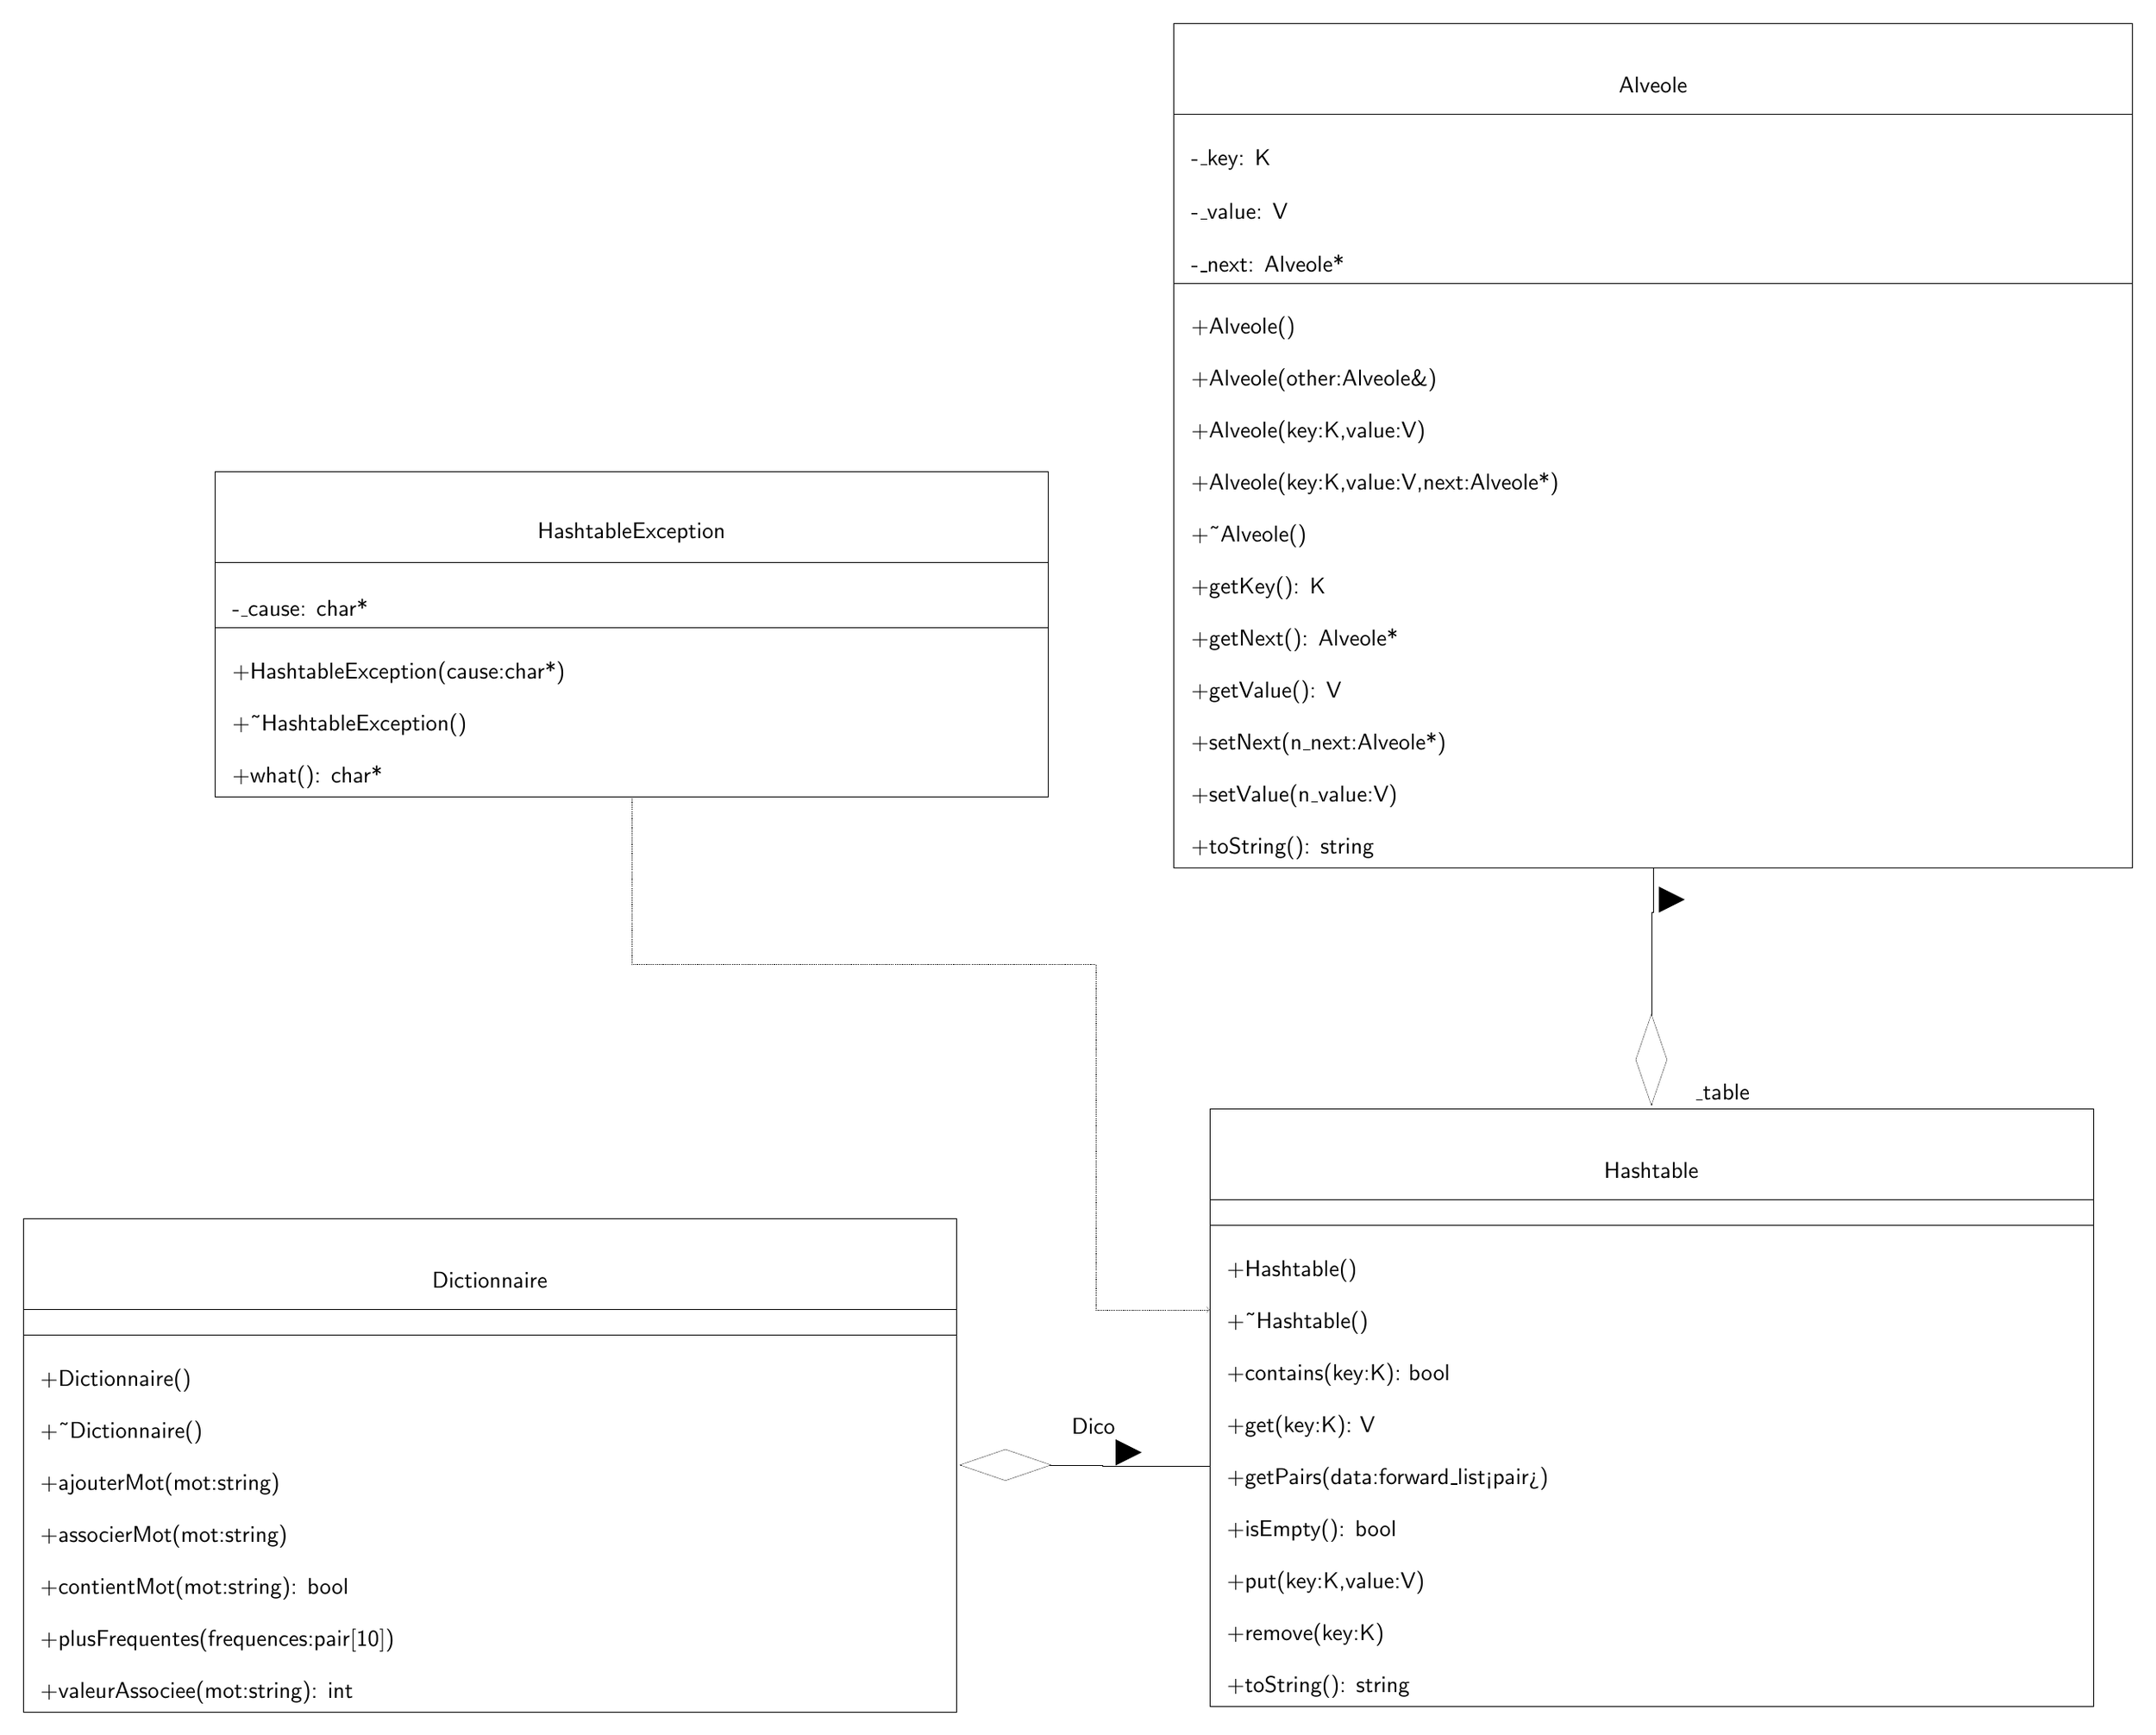
\begin{tikzpicture}
\pgftransformxscale{1.000000}
\pgftransformyscale{-1.000000}
\definecolor{dialinecolor}{rgb}{0.000000, 0.000000, 0.000000}
\pgfsetstrokecolor{dialinecolor}
\definecolor{dialinecolor}{rgb}{1.000000, 1.000000, 1.000000}
\pgfsetfillcolor{dialinecolor}
\pgfsetlinewidth{0.100000\du}
\pgfsetdash{}{0pt}
\definecolor{dialinecolor}{rgb}{1.000000, 1.000000, 1.000000}
\pgfsetfillcolor{dialinecolor}
\fill (4.800000\du,8.750000\du)--(4.800000\du,10.150000\du)--(17.620000\du,10.150000\du)--(17.620000\du,8.750000\du)--cycle;
\definecolor{dialinecolor}{rgb}{0.000000, 0.000000, 0.000000}
\pgfsetstrokecolor{dialinecolor}
\draw (4.800000\du,8.750000\du)--(4.800000\du,10.150000\du)--(17.620000\du,10.150000\du)--(17.620000\du,8.750000\du)--cycle;
% setfont left to latex
\definecolor{dialinecolor}{rgb}{0.000000, 0.000000, 0.000000}
\pgfsetstrokecolor{dialinecolor}
\node at (11.210000\du,9.700000\du){HashtableException};
\definecolor{dialinecolor}{rgb}{1.000000, 1.000000, 1.000000}
\pgfsetfillcolor{dialinecolor}
\fill (4.800000\du,10.150000\du)--(4.800000\du,11.150000\du)--(17.620000\du,11.150000\du)--(17.620000\du,10.150000\du)--cycle;
\definecolor{dialinecolor}{rgb}{0.000000, 0.000000, 0.000000}
\pgfsetstrokecolor{dialinecolor}
\draw (4.800000\du,10.150000\du)--(4.800000\du,11.150000\du)--(17.620000\du,11.150000\du)--(17.620000\du,10.150000\du)--cycle;
% setfont left to latex
\definecolor{dialinecolor}{rgb}{0.000000, 0.000000, 0.000000}
\pgfsetstrokecolor{dialinecolor}
\node[anchor=west] at (4.950000\du,10.850000\du){-\_cause: char*};
\definecolor{dialinecolor}{rgb}{1.000000, 1.000000, 1.000000}
\pgfsetfillcolor{dialinecolor}
\fill (4.800000\du,11.150000\du)--(4.800000\du,13.750000\du)--(17.620000\du,13.750000\du)--(17.620000\du,11.150000\du)--cycle;
\definecolor{dialinecolor}{rgb}{0.000000, 0.000000, 0.000000}
\pgfsetstrokecolor{dialinecolor}
\draw (4.800000\du,11.150000\du)--(4.800000\du,13.750000\du)--(17.620000\du,13.750000\du)--(17.620000\du,11.150000\du)--cycle;
% setfont left to latex
\definecolor{dialinecolor}{rgb}{0.000000, 0.000000, 0.000000}
\pgfsetstrokecolor{dialinecolor}
\node[anchor=west] at (4.950000\du,11.850000\du){+HashtableException(cause:char*)};
% setfont left to latex
\definecolor{dialinecolor}{rgb}{0.000000, 0.000000, 0.000000}
\pgfsetstrokecolor{dialinecolor}
\node[anchor=west] at (4.950000\du,12.650000\du){+\~{}HashtableException()};
% setfont left to latex
\definecolor{dialinecolor}{rgb}{0.000000, 0.000000, 0.000000}
\pgfsetstrokecolor{dialinecolor}
\node[anchor=west] at (4.950000\du,13.450000\du){+what(): char*};
\pgfsetlinewidth{0.100000\du}
\pgfsetdash{}{0pt}
\definecolor{dialinecolor}{rgb}{1.000000, 1.000000, 1.000000}
\pgfsetfillcolor{dialinecolor}
\fill (19.550000\du,1.850000\du)--(19.550000\du,3.250000\du)--(34.295000\du,3.250000\du)--(34.295000\du,1.850000\du)--cycle;
\definecolor{dialinecolor}{rgb}{0.000000, 0.000000, 0.000000}
\pgfsetstrokecolor{dialinecolor}
\draw (19.550000\du,1.850000\du)--(19.550000\du,3.250000\du)--(34.295000\du,3.250000\du)--(34.295000\du,1.850000\du)--cycle;
% setfont left to latex
\definecolor{dialinecolor}{rgb}{0.000000, 0.000000, 0.000000}
\pgfsetstrokecolor{dialinecolor}
\node at (26.922500\du,2.800000\du){Alveole};
\definecolor{dialinecolor}{rgb}{1.000000, 1.000000, 1.000000}
\pgfsetfillcolor{dialinecolor}
\fill (19.550000\du,3.250000\du)--(19.550000\du,5.850000\du)--(34.295000\du,5.850000\du)--(34.295000\du,3.250000\du)--cycle;
\definecolor{dialinecolor}{rgb}{0.000000, 0.000000, 0.000000}
\pgfsetstrokecolor{dialinecolor}
\draw (19.550000\du,3.250000\du)--(19.550000\du,5.850000\du)--(34.295000\du,5.850000\du)--(34.295000\du,3.250000\du)--cycle;
% setfont left to latex
\definecolor{dialinecolor}{rgb}{0.000000, 0.000000, 0.000000}
\pgfsetstrokecolor{dialinecolor}
\node[anchor=west] at (19.700000\du,3.950000\du){-\_key: K};
% setfont left to latex
\definecolor{dialinecolor}{rgb}{0.000000, 0.000000, 0.000000}
\pgfsetstrokecolor{dialinecolor}
\node[anchor=west] at (19.700000\du,4.750000\du){-\_value: V};
% setfont left to latex
\definecolor{dialinecolor}{rgb}{0.000000, 0.000000, 0.000000}
\pgfsetstrokecolor{dialinecolor}
\node[anchor=west] at (19.700000\du,5.550000\du){-\_next: Alveole*};
\definecolor{dialinecolor}{rgb}{1.000000, 1.000000, 1.000000}
\pgfsetfillcolor{dialinecolor}
\fill (19.550000\du,5.850000\du)--(19.550000\du,14.850000\du)--(34.295000\du,14.850000\du)--(34.295000\du,5.850000\du)--cycle;
\definecolor{dialinecolor}{rgb}{0.000000, 0.000000, 0.000000}
\pgfsetstrokecolor{dialinecolor}
\draw (19.550000\du,5.850000\du)--(19.550000\du,14.850000\du)--(34.295000\du,14.850000\du)--(34.295000\du,5.850000\du)--cycle;
% setfont left to latex
\definecolor{dialinecolor}{rgb}{0.000000, 0.000000, 0.000000}
\pgfsetstrokecolor{dialinecolor}
\node[anchor=west] at (19.700000\du,6.550000\du){+Alveole()};
% setfont left to latex
\definecolor{dialinecolor}{rgb}{0.000000, 0.000000, 0.000000}
\pgfsetstrokecolor{dialinecolor}
\node[anchor=west] at (19.700000\du,7.350000\du){+Alveole(other:Alveole\&)};
% setfont left to latex
\definecolor{dialinecolor}{rgb}{0.000000, 0.000000, 0.000000}
\pgfsetstrokecolor{dialinecolor}
\node[anchor=west] at (19.700000\du,8.150000\du){+Alveole(key:K,value:V)};
% setfont left to latex
\definecolor{dialinecolor}{rgb}{0.000000, 0.000000, 0.000000}
\pgfsetstrokecolor{dialinecolor}
\node[anchor=west] at (19.700000\du,8.950000\du){+Alveole(key:K,value:V,next:Alveole*)};
% setfont left to latex
\definecolor{dialinecolor}{rgb}{0.000000, 0.000000, 0.000000}
\pgfsetstrokecolor{dialinecolor}
\node[anchor=west] at (19.700000\du,9.750000\du){+\~{}Alveole()};
% setfont left to latex
\definecolor{dialinecolor}{rgb}{0.000000, 0.000000, 0.000000}
\pgfsetstrokecolor{dialinecolor}
\node[anchor=west] at (19.700000\du,10.550000\du){+getKey(): K};
% setfont left to latex
\definecolor{dialinecolor}{rgb}{0.000000, 0.000000, 0.000000}
\pgfsetstrokecolor{dialinecolor}
\node[anchor=west] at (19.700000\du,11.350000\du){+getNext(): Alveole*};
% setfont left to latex
\definecolor{dialinecolor}{rgb}{0.000000, 0.000000, 0.000000}
\pgfsetstrokecolor{dialinecolor}
\node[anchor=west] at (19.700000\du,12.150000\du){+getValue(): V};
% setfont left to latex
\definecolor{dialinecolor}{rgb}{0.000000, 0.000000, 0.000000}
\pgfsetstrokecolor{dialinecolor}
\node[anchor=west] at (19.700000\du,12.950000\du){+setNext(n\_next:Alveole*)};
% setfont left to latex
\definecolor{dialinecolor}{rgb}{0.000000, 0.000000, 0.000000}
\pgfsetstrokecolor{dialinecolor}
\node[anchor=west] at (19.700000\du,13.750000\du){+setValue(n\_value:V)};
% setfont left to latex
\definecolor{dialinecolor}{rgb}{0.000000, 0.000000, 0.000000}
\pgfsetstrokecolor{dialinecolor}
\node[anchor=west] at (19.700000\du,14.550000\du){+toString(): string};
\pgfsetlinewidth{0.100000\du}
\pgfsetdash{}{0pt}
\definecolor{dialinecolor}{rgb}{1.000000, 1.000000, 1.000000}
\pgfsetfillcolor{dialinecolor}
\fill (20.100000\du,18.550000\du)--(20.100000\du,19.950000\du)--(33.690000\du,19.950000\du)--(33.690000\du,18.550000\du)--cycle;
\definecolor{dialinecolor}{rgb}{0.000000, 0.000000, 0.000000}
\pgfsetstrokecolor{dialinecolor}
\draw (20.100000\du,18.550000\du)--(20.100000\du,19.950000\du)--(33.690000\du,19.950000\du)--(33.690000\du,18.550000\du)--cycle;
% setfont left to latex
\definecolor{dialinecolor}{rgb}{0.000000, 0.000000, 0.000000}
\pgfsetstrokecolor{dialinecolor}
\node at (26.895000\du,19.500000\du){Hashtable};
\definecolor{dialinecolor}{rgb}{1.000000, 1.000000, 1.000000}
\pgfsetfillcolor{dialinecolor}
\fill (20.100000\du,19.950000\du)--(20.100000\du,20.350000\du)--(33.690000\du,20.350000\du)--(33.690000\du,19.950000\du)--cycle;
\definecolor{dialinecolor}{rgb}{0.000000, 0.000000, 0.000000}
\pgfsetstrokecolor{dialinecolor}
\draw (20.100000\du,19.950000\du)--(20.100000\du,20.350000\du)--(33.690000\du,20.350000\du)--(33.690000\du,19.950000\du)--cycle;
\definecolor{dialinecolor}{rgb}{1.000000, 1.000000, 1.000000}
\pgfsetfillcolor{dialinecolor}
\fill (20.100000\du,20.350000\du)--(20.100000\du,27.750000\du)--(33.690000\du,27.750000\du)--(33.690000\du,20.350000\du)--cycle;
\definecolor{dialinecolor}{rgb}{0.000000, 0.000000, 0.000000}
\pgfsetstrokecolor{dialinecolor}
\draw (20.100000\du,20.350000\du)--(20.100000\du,27.750000\du)--(33.690000\du,27.750000\du)--(33.690000\du,20.350000\du)--cycle;
% setfont left to latex
\definecolor{dialinecolor}{rgb}{0.000000, 0.000000, 0.000000}
\pgfsetstrokecolor{dialinecolor}
\node[anchor=west] at (20.250000\du,21.050000\du){+Hashtable()};
% setfont left to latex
\definecolor{dialinecolor}{rgb}{0.000000, 0.000000, 0.000000}
\pgfsetstrokecolor{dialinecolor}
\node[anchor=west] at (20.250000\du,21.850000\du){+\~{}Hashtable()};
% setfont left to latex
\definecolor{dialinecolor}{rgb}{0.000000, 0.000000, 0.000000}
\pgfsetstrokecolor{dialinecolor}
\node[anchor=west] at (20.250000\du,22.650000\du){+contains(key:K): bool};
% setfont left to latex
\definecolor{dialinecolor}{rgb}{0.000000, 0.000000, 0.000000}
\pgfsetstrokecolor{dialinecolor}
\node[anchor=west] at (20.250000\du,23.450000\du){+get(key:K): V};
% setfont left to latex
\definecolor{dialinecolor}{rgb}{0.000000, 0.000000, 0.000000}
\pgfsetstrokecolor{dialinecolor}
\node[anchor=west] at (20.250000\du,24.250000\du){+getPairs(data:forward\_list<pair>)};
% setfont left to latex
\definecolor{dialinecolor}{rgb}{0.000000, 0.000000, 0.000000}
\pgfsetstrokecolor{dialinecolor}
\node[anchor=west] at (20.250000\du,25.050000\du){+isEmpty(): bool};
% setfont left to latex
\definecolor{dialinecolor}{rgb}{0.000000, 0.000000, 0.000000}
\pgfsetstrokecolor{dialinecolor}
\node[anchor=west] at (20.250000\du,25.850000\du){+put(key:K,value:V)};
% setfont left to latex
\definecolor{dialinecolor}{rgb}{0.000000, 0.000000, 0.000000}
\pgfsetstrokecolor{dialinecolor}
\node[anchor=west] at (20.250000\du,26.650000\du){+remove(key:K)};
% setfont left to latex
\definecolor{dialinecolor}{rgb}{0.000000, 0.000000, 0.000000}
\pgfsetstrokecolor{dialinecolor}
\node[anchor=west] at (20.250000\du,27.450000\du){+toString(): string};
\pgfsetlinewidth{0.100000\du}
\pgfsetdash{{1.000000\du}{1.000000\du}}{0\du}
\pgfsetdash{{0.400000\du}{0.400000\du}}{0\du}
\pgfsetmiterjoin
\pgfsetbuttcap
{
\definecolor{dialinecolor}{rgb}{0.000000, 0.000000, 0.000000}
\pgfsetfillcolor{dialinecolor}
% was here!!!
\pgfsetarrowsend{to}
\definecolor{dialinecolor}{rgb}{0.000000, 0.000000, 0.000000}
\pgfsetstrokecolor{dialinecolor}
\draw (11.210000\du,13.750000\du)--(11.210000\du,16.337500\du)--(18.350000\du,16.337500\du)--(18.350000\du,21.650000\du)--(20.100000\du,21.650000\du);
}
% setfont left to latex
\pgfsetlinewidth{0.100000\du}
\pgfsetdash{}{0pt}
\pgfsetmiterjoin
\pgfsetbuttcap
{
\definecolor{dialinecolor}{rgb}{0.000000, 0.000000, 0.000000}
\pgfsetfillcolor{dialinecolor}
% was here!!!
\definecolor{dialinecolor}{rgb}{0.000000, 0.000000, 0.000000}
\pgfsetstrokecolor{dialinecolor}
\draw (26.895000\du,18.501840\du)--(26.895000\du,15.537500\du)--(26.922500\du,15.537500\du)--(26.922500\du,14.850000\du);
}
\definecolor{dialinecolor}{rgb}{0.000000, 0.000000, 0.000000}
\pgfsetstrokecolor{dialinecolor}
\draw (26.895000\du,17.243262\du)--(26.895000\du,15.537500\du)--(26.922500\du,15.537500\du)--(26.922500\du,14.850000\du);
\pgfsetdash{}{0pt}
\pgfsetmiterjoin
\pgfsetbuttcap
\definecolor{dialinecolor}{rgb}{1.000000, 1.000000, 1.000000}
\pgfsetfillcolor{dialinecolor}
\fill (26.895000\du,18.501840\du)--(26.655000\du,17.801840\du)--(26.895000\du,17.101840\du)--(27.135000\du,17.801840\du)--cycle;
\pgfsetlinewidth{0.100000\du}
\pgfsetdash{}{0pt}
\pgfsetmiterjoin
\pgfsetbuttcap
\definecolor{dialinecolor}{rgb}{0.000000, 0.000000, 0.000000}
\pgfsetstrokecolor{dialinecolor}
\draw (26.895000\du,18.501840\du)--(26.655000\du,17.801840\du)--(26.895000\du,17.101840\du)--(27.135000\du,17.801840\du)--cycle;
% setfont left to latex
\definecolor{dialinecolor}{rgb}{0.000000, 0.000000, 0.000000}
\pgfsetfillcolor{dialinecolor}
\fill (27.008750\du,15.537500\du)--(27.008750\du,15.137500\du)--(27.408750\du,15.337500\du)--cycle;
\definecolor{dialinecolor}{rgb}{0.000000, 0.000000, 0.000000}
\pgfsetstrokecolor{dialinecolor}
\node[anchor=west] at (27.445000\du,18.301840\du){ \_table};
\pgfsetlinewidth{0.100000\du}
\pgfsetdash{}{0pt}
\definecolor{dialinecolor}{rgb}{1.000000, 1.000000, 1.000000}
\pgfsetfillcolor{dialinecolor}
\fill (1.850000\du,20.237500\du)--(1.850000\du,21.637500\du)--(16.210000\du,21.637500\du)--(16.210000\du,20.237500\du)--cycle;
\definecolor{dialinecolor}{rgb}{0.000000, 0.000000, 0.000000}
\pgfsetstrokecolor{dialinecolor}
\draw (1.850000\du,20.237500\du)--(1.850000\du,21.637500\du)--(16.210000\du,21.637500\du)--(16.210000\du,20.237500\du)--cycle;
% setfont left to latex
\definecolor{dialinecolor}{rgb}{0.000000, 0.000000, 0.000000}
\pgfsetstrokecolor{dialinecolor}
\node at (9.030000\du,21.187500\du){Dictionnaire};
\definecolor{dialinecolor}{rgb}{1.000000, 1.000000, 1.000000}
\pgfsetfillcolor{dialinecolor}
\fill (1.850000\du,21.637500\du)--(1.850000\du,22.037500\du)--(16.210000\du,22.037500\du)--(16.210000\du,21.637500\du)--cycle;
\definecolor{dialinecolor}{rgb}{0.000000, 0.000000, 0.000000}
\pgfsetstrokecolor{dialinecolor}
\draw (1.850000\du,21.637500\du)--(1.850000\du,22.037500\du)--(16.210000\du,22.037500\du)--(16.210000\du,21.637500\du)--cycle;
\definecolor{dialinecolor}{rgb}{1.000000, 1.000000, 1.000000}
\pgfsetfillcolor{dialinecolor}
\fill (1.850000\du,22.037500\du)--(1.850000\du,27.837500\du)--(16.210000\du,27.837500\du)--(16.210000\du,22.037500\du)--cycle;
\definecolor{dialinecolor}{rgb}{0.000000, 0.000000, 0.000000}
\pgfsetstrokecolor{dialinecolor}
\draw (1.850000\du,22.037500\du)--(1.850000\du,27.837500\du)--(16.210000\du,27.837500\du)--(16.210000\du,22.037500\du)--cycle;
% setfont left to latex
\definecolor{dialinecolor}{rgb}{0.000000, 0.000000, 0.000000}
\pgfsetstrokecolor{dialinecolor}
\node[anchor=west] at (2.000000\du,22.737500\du){+Dictionnaire()};
% setfont left to latex
\definecolor{dialinecolor}{rgb}{0.000000, 0.000000, 0.000000}
\pgfsetstrokecolor{dialinecolor}
\node[anchor=west] at (2.000000\du,23.537500\du){+\~{}Dictionnaire()};
% setfont left to latex
\definecolor{dialinecolor}{rgb}{0.000000, 0.000000, 0.000000}
\pgfsetstrokecolor{dialinecolor}
\node[anchor=west] at (2.000000\du,24.337500\du){+ajouterMot(mot:string)};
% setfont left to latex
\definecolor{dialinecolor}{rgb}{0.000000, 0.000000, 0.000000}
\pgfsetstrokecolor{dialinecolor}
\node[anchor=west] at (2.000000\du,25.137500\du){+associerMot(mot:string)};
% setfont left to latex
\definecolor{dialinecolor}{rgb}{0.000000, 0.000000, 0.000000}
\pgfsetstrokecolor{dialinecolor}
\node[anchor=west] at (2.000000\du,25.937500\du){+contientMot(mot:string): bool};
% setfont left to latex
\definecolor{dialinecolor}{rgb}{0.000000, 0.000000, 0.000000}
\pgfsetstrokecolor{dialinecolor}
\node[anchor=west] at (2.000000\du,26.737500\du){+plusFrequentes(frequences:pair\ensuremath{[}10\ensuremath{]})};
% setfont left to latex
\definecolor{dialinecolor}{rgb}{0.000000, 0.000000, 0.000000}
\pgfsetstrokecolor{dialinecolor}
\node[anchor=west] at (2.000000\du,27.537500\du){+valeurAssociee(mot:string): int};
\pgfsetlinewidth{0.100000\du}
\pgfsetdash{}{0pt}
\pgfsetmiterjoin
\pgfsetbuttcap
{
\definecolor{dialinecolor}{rgb}{0.000000, 0.000000, 0.000000}
\pgfsetfillcolor{dialinecolor}
% was here!!!
\definecolor{dialinecolor}{rgb}{0.000000, 0.000000, 0.000000}
\pgfsetstrokecolor{dialinecolor}
\draw (16.260406\du,24.037500\du)--(18.455012\du,24.037500\du)--(18.455012\du,24.050000\du)--(20.100000\du,24.050000\du);
}
\definecolor{dialinecolor}{rgb}{0.000000, 0.000000, 0.000000}
\pgfsetstrokecolor{dialinecolor}
\draw (17.518985\du,24.037500\du)--(18.455012\du,24.037500\du)--(18.455012\du,24.050000\du)--(20.100000\du,24.050000\du);
\pgfsetdash{}{0pt}
\pgfsetmiterjoin
\pgfsetbuttcap
\definecolor{dialinecolor}{rgb}{1.000000, 1.000000, 1.000000}
\pgfsetfillcolor{dialinecolor}
\fill (16.260406\du,24.037500\du)--(16.960406\du,23.797500\du)--(17.660406\du,24.037500\du)--(16.960406\du,24.277500\du)--cycle;
\pgfsetlinewidth{0.100000\du}
\pgfsetdash{}{0pt}
\pgfsetmiterjoin
\pgfsetbuttcap
\definecolor{dialinecolor}{rgb}{0.000000, 0.000000, 0.000000}
\pgfsetstrokecolor{dialinecolor}
\draw (16.260406\du,24.037500\du)--(16.960406\du,23.797500\du)--(17.660406\du,24.037500\du)--(16.960406\du,24.277500\du)--cycle;
% setfont left to latex
\definecolor{dialinecolor}{rgb}{0.000000, 0.000000, 0.000000}
\pgfsetfillcolor{dialinecolor}
\fill (18.655012\du,24.043750\du)--(18.655012\du,23.643750\du)--(19.055012\du,23.843750\du)--cycle;
\definecolor{dialinecolor}{rgb}{0.000000, 0.000000, 0.000000}
\pgfsetstrokecolor{dialinecolor}
\node[anchor=west] at (17.860406\du,23.437500\du){ Dico};
\end{tikzpicture}

\hypertarget{class_hashtable_exception}{\section{Hashtable\-Exception Class Reference}
\label{class_hashtable_exception}\index{Hashtable\-Exception@{Hashtable\-Exception}}
}


Exception class to manage \hyperlink{class_hashtable}{Hashtable} errors.  




{\ttfamily \#include $<$hashtable.\-hpp$>$}

Inheritance diagram for Hashtable\-Exception\-:\begin{figure}[H]
\begin{center}
\leavevmode
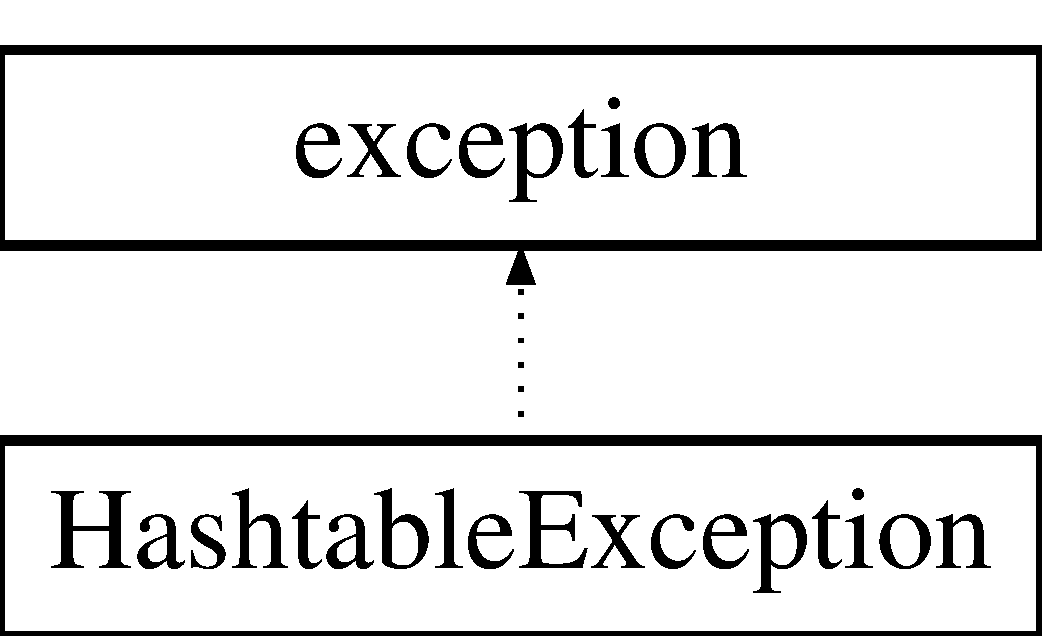
\includegraphics[height=2.000000cm]{class_hashtable_exception}
\end{center}
\end{figure}
\subsection*{Public Member Functions}
\begin{DoxyCompactItemize}
\item 
\hyperlink{class_hashtable_exception_a1a3ae95bd655064144b485f0938fddca}{Hashtable\-Exception} (const char $\ast$cause)
\item 
virtual \hyperlink{class_hashtable_exception_a9668a272e0470e9d4a16f0f5307e6153}{$\sim$\-Hashtable\-Exception} ()  throw ()
\item 
virtual const char $\ast$ \hyperlink{class_hashtable_exception_a980d0861fe744622043fcdd654ea5e07}{what} () const   throw ()
\end{DoxyCompactItemize}
\subsection*{Private Attributes}
\begin{DoxyCompactItemize}
\item 
const char $\ast$ \hyperlink{class_hashtable_exception_a242dcd5048ce89c2aadd0ca97f5c6d9a}{\-\_\-cause}
\end{DoxyCompactItemize}


\subsection{Detailed Description}
Exception class to manage \hyperlink{class_hashtable}{Hashtable} errors. 

\subsection{Constructor \& Destructor Documentation}
\hypertarget{class_hashtable_exception_a1a3ae95bd655064144b485f0938fddca}{\index{Hashtable\-Exception@{Hashtable\-Exception}!Hashtable\-Exception@{Hashtable\-Exception}}
\index{Hashtable\-Exception@{Hashtable\-Exception}!HashtableException@{Hashtable\-Exception}}
\subsubsection[{Hashtable\-Exception}]{\setlength{\rightskip}{0pt plus 5cm}Hashtable\-Exception\-::\-Hashtable\-Exception (
\begin{DoxyParamCaption}
\item[{const char $\ast$}]{cause}
\end{DoxyParamCaption}
)}}\label{class_hashtable_exception_a1a3ae95bd655064144b485f0938fddca}
store exception description constructor called then Hashtable\-Exceptions are threw 
\begin{DoxyParams}[1]{Parameters}
\mbox{\tt in}  & {\em cause} & description of exception origin \\
\hline
\end{DoxyParams}
\hypertarget{class_hashtable_exception_a9668a272e0470e9d4a16f0f5307e6153}{\index{Hashtable\-Exception@{Hashtable\-Exception}!$\sim$\-Hashtable\-Exception@{$\sim$\-Hashtable\-Exception}}
\index{$\sim$\-Hashtable\-Exception@{$\sim$\-Hashtable\-Exception}!HashtableException@{Hashtable\-Exception}}
\subsubsection[{$\sim$\-Hashtable\-Exception}]{\setlength{\rightskip}{0pt plus 5cm}virtual Hashtable\-Exception\-::$\sim$\-Hashtable\-Exception (
\begin{DoxyParamCaption}
{}
\end{DoxyParamCaption}
) throw  ) \hspace{0.3cm}{\ttfamily [virtual]}}}\label{class_hashtable_exception_a9668a272e0470e9d4a16f0f5307e6153}
destructor currently, do anything special 

\subsection{Member Function Documentation}
\hypertarget{class_hashtable_exception_a980d0861fe744622043fcdd654ea5e07}{\index{Hashtable\-Exception@{Hashtable\-Exception}!what@{what}}
\index{what@{what}!HashtableException@{Hashtable\-Exception}}
\subsubsection[{what}]{\setlength{\rightskip}{0pt plus 5cm}virtual const char$\ast$ Hashtable\-Exception\-::what (
\begin{DoxyParamCaption}
{}
\end{DoxyParamCaption}
) const throw  ) \hspace{0.3cm}{\ttfamily [virtual]}}}\label{class_hashtable_exception_a980d0861fe744622043fcdd654ea5e07}
virtual fonction from superclass, usefull to get the exception description 

\subsection{Member Data Documentation}
\hypertarget{class_hashtable_exception_a242dcd5048ce89c2aadd0ca97f5c6d9a}{\index{Hashtable\-Exception@{Hashtable\-Exception}!\-\_\-cause@{\-\_\-cause}}
\index{\-\_\-cause@{\-\_\-cause}!HashtableException@{Hashtable\-Exception}}
\subsubsection[{\-\_\-cause}]{\setlength{\rightskip}{0pt plus 5cm}const char$\ast$ Hashtable\-Exception\-::\-\_\-cause\hspace{0.3cm}{\ttfamily [private]}}}\label{class_hashtable_exception_a242dcd5048ce89c2aadd0ca97f5c6d9a}


The documentation for this class was generated from the following file\-:\begin{DoxyCompactItemize}
\item 
src/\hyperlink{hashtable_8hpp}{hashtable.\-hpp}\end{DoxyCompactItemize}

\hypertarget{class_node}{\section{Node$<$ T $>$ Class Template Reference}
\label{class_node}\index{Node$<$ T $>$@{Node$<$ T $>$}}
}


Defines tree nodes.  




{\ttfamily \#include $<$tree.\-hpp$>$}

\subsection*{Public Member Functions}
\begin{DoxyCompactItemize}
\item 
\hyperlink{class_node_ad70e3545b2df020088a0e26bec128632}{Node} (const \hyperlink{class_node}{Node}$<$ T $>$ \&other)
\item 
\hyperlink{class_node_a0692b16d246460bf94c18d49592facdd}{Node} (T data)
\item 
\hyperlink{class_node_ae923d0417581dd19784d55b901f0f7f0}{$\sim$\-Node} ()
\item 
\hyperlink{class_node}{Node}$<$ T $>$ \& \hyperlink{class_node_aa9d37ee4133ae9774c5cf2ca5a6da8af}{operator=} (\hyperlink{class_node}{Node}$<$ T $>$ \&other)
\item 
bool \hyperlink{class_node_ac6af63bbc9a1eef28615c5c0c5acb83c}{operator==} (const \hyperlink{class_node}{Node}$<$ T $>$ \&rhs)
\item 
bool \hyperlink{class_node_acb50abe854f383e0d624e85505697b4f}{operator!=} (const \hyperlink{class_node}{Node}$<$ T $>$ \&rhs)
\item 
bool \hyperlink{class_node_a26f91ff0b0d5ea8940c7fde220aca742}{is\-Leaf} ()
\item 
int \hyperlink{class_node_a0da7f6a2356d1e7f047f8bfda1edd8d8}{height} ()
\item 
void \hyperlink{class_node_a141b357c5d9a30cd9b3062337ef67edb}{append} (T n\-\_\-data)
\item 
void \hyperlink{class_node_a33901811ec542883fdfc68022dd59920}{remove} (T data)
\item 
T \hyperlink{class_node_a3b188b785e394924c11f2f68369c0cdf}{get\-Tag} ()
\item 
bool \hyperlink{class_node_ad319e53c90ce8bced6ffc42b67d8e759}{contains} (T element)
\item 
string \hyperlink{class_node_abb91d745a01f97fe51a35811e0d42801}{to\-String} ()
\item 
\hyperlink{class_node_a95419c19d47e2521d437b81768c3896e}{Node} (const \hyperlink{class_node}{Node} \&other)
\item 
\hyperlink{class_node_a42c85c1e6abbc2999f85cf19dd8bc7c2}{Node} (char data, int frequency)
\item 
\hyperlink{class_node_a0ac1d44cfe588be564acf25485029bd8}{Node} ()
\item 
\hyperlink{class_node_ae923d0417581dd19784d55b901f0f7f0}{$\sim$\-Node} ()
\item 
\hyperlink{class_node}{Node} \& \hyperlink{class_node_aeacd56499cfe37836344a2eb679490f4}{operator=} (const \hyperlink{class_node}{Node} \&other)
\item 
bool \hyperlink{class_node_adcebaf614477737c439128517415f799}{operator==} (const \hyperlink{class_node}{Node} \&rhs)
\item 
bool \hyperlink{class_node_a9ae22944b815b5f95bc5f31f9f6b41ab}{operator!=} (const \hyperlink{class_node}{Node} \&rhs)
\item 
bool \hyperlink{class_node_a26f91ff0b0d5ea8940c7fde220aca742}{is\-Leaf} ()
\item 
int \hyperlink{class_node_a0da7f6a2356d1e7f047f8bfda1edd8d8}{height} ()
\item 
\hyperlink{class_node}{Node} $\ast$ \hyperlink{class_node_ac175219981b8633f47f6a93f6271cd91}{append} (const char n\-\_\-data, int frequency)
\item 
char \hyperlink{class_node_affb5abc8a7422a40c44deba0a79a10cf}{get\-Tag} ()
\item 
string \hyperlink{class_node_abb91d745a01f97fe51a35811e0d42801}{to\-String} ()
\item 
void \hyperlink{class_node_acca1581b1ffc18b14ac92073d932c099}{to\-List} (forward\-\_\-list$<$ string $>$ \&words, string word)
\item 
void \hyperlink{class_node_ae8592b9ab27d013cf6acc6efacb39d1a}{to\-Frequenced\-List} (forward\-\_\-list$<$ pair$<$ string, int $>$$>$ \&words, string word)
\end{DoxyCompactItemize}
\subsection*{Private Attributes}
\begin{DoxyCompactItemize}
\item 
int \hyperlink{class_node_a4b3606724f7302e3df96ff87d623312d}{\-\_\-child\-Nbr}
\begin{DoxyCompactList}\small\item\em Number of children. \end{DoxyCompactList}\item 
T \hyperlink{class_node_a82089b860871012bc159c510408be29c}{\-\_\-tag}
\begin{DoxyCompactList}\small\item\em letter stored into \hyperlink{class_node}{Node}, the tag \end{DoxyCompactList}\item 
forward\-\_\-list$<$ \hyperlink{class_node}{Node}$<$ T $>$ $>$ \hyperlink{class_node_a845317829093b3d4665ba7e0055b4599}{\-\_\-children}
\begin{DoxyCompactList}\small\item\em children of the \hyperlink{class_node}{Node} \end{DoxyCompactList}\item 
int \hyperlink{class_node_add728cb28da68ec5ef2d9cac31c9a08d}{\-\_\-word\-Frequency}
\item 
char \hyperlink{class_node_a24a667af4a37caad6e15b94fb76885b1}{\-\_\-tag}
\begin{DoxyCompactList}\small\item\em letter stored into \hyperlink{class_node}{Node}, the tag \end{DoxyCompactList}\item 
forward\-\_\-list$<$ \hyperlink{class_node}{Node} $\ast$ $>$ \hyperlink{class_node_ac4c86c8bbc999016827248dbe8b7cc96}{\-\_\-children}
\begin{DoxyCompactList}\small\item\em children of the \hyperlink{class_node}{Node} \end{DoxyCompactList}\end{DoxyCompactItemize}


\subsection{Detailed Description}
\subsubsection*{template$<$typename T = char$>$class Node$<$ T $>$}

Defines tree nodes. 

Class for nodes of a tree. A \hyperlink{class_node}{Node} store a tag and can have several children

Class for nodes of a \hyperlink{class_tree_string}{Tree\-String}. A \hyperlink{class_node}{Node} store a letter and can have several children. 

\subsection{Constructor \& Destructor Documentation}
\hypertarget{class_node_ad70e3545b2df020088a0e26bec128632}{\index{Node@{Node}!Node@{Node}}
\index{Node@{Node}!Node@{Node}}
\subsubsection[{Node}]{\setlength{\rightskip}{0pt plus 5cm}template$<$typename T = char$>$ {\bf Node}$<$ T $>$\-::{\bf Node} (
\begin{DoxyParamCaption}
\item[{const {\bf Node}$<$ T $>$ \&}]{other}
\end{DoxyParamCaption}
)}}\label{class_node_ad70e3545b2df020088a0e26bec128632}
Copy constructor 
\begin{DoxyParams}[1]{Parameters}
\mbox{\tt in}  & {\em other} & \hyperlink{class_node}{Node} to copy \\
\hline
\end{DoxyParams}
\hypertarget{class_node_a0692b16d246460bf94c18d49592facdd}{\index{Node@{Node}!Node@{Node}}
\index{Node@{Node}!Node@{Node}}
\subsubsection[{Node}]{\setlength{\rightskip}{0pt plus 5cm}template$<$typename T = char$>$ {\bf Node}$<$ T $>$\-::{\bf Node} (
\begin{DoxyParamCaption}
\item[{T}]{data}
\end{DoxyParamCaption}
)}}\label{class_node_a0692b16d246460bf94c18d49592facdd}
Simple constructor 
\begin{DoxyParams}[1]{Parameters}
\mbox{\tt in}  & {\em data} & to store into the \hyperlink{class_node}{Node} \\
\hline
\end{DoxyParams}
\hypertarget{class_node_ae923d0417581dd19784d55b901f0f7f0}{\index{Node@{Node}!$\sim$\-Node@{$\sim$\-Node}}
\index{$\sim$\-Node@{$\sim$\-Node}!Node@{Node}}
\subsubsection[{$\sim$\-Node}]{\setlength{\rightskip}{0pt plus 5cm}template$<$typename T = char$>$ {\bf Node}$<$ T $>$\-::$\sim${\bf Node} (
\begin{DoxyParamCaption}
{}
\end{DoxyParamCaption}
)}}\label{class_node_ae923d0417581dd19784d55b901f0f7f0}
Destructor for \hyperlink{class_node}{Node} \hypertarget{class_node_a95419c19d47e2521d437b81768c3896e}{\index{Node@{Node}!Node@{Node}}
\index{Node@{Node}!Node@{Node}}
\subsubsection[{Node}]{\setlength{\rightskip}{0pt plus 5cm}template$<$typename T = char$>$ {\bf Node}$<$ T $>$\-::{\bf Node} (
\begin{DoxyParamCaption}
\item[{const {\bf Node}$<$ T $>$ \&}]{other}
\end{DoxyParamCaption}
)}}\label{class_node_a95419c19d47e2521d437b81768c3896e}
Copy constructor 
\begin{DoxyParams}[1]{Parameters}
\mbox{\tt in}  & {\em other} & \hyperlink{class_node}{Node} to copy \\
\hline
\end{DoxyParams}
\hypertarget{class_node_a42c85c1e6abbc2999f85cf19dd8bc7c2}{\index{Node@{Node}!Node@{Node}}
\index{Node@{Node}!Node@{Node}}
\subsubsection[{Node}]{\setlength{\rightskip}{0pt plus 5cm}template$<$typename T = char$>$ {\bf Node}$<$ T $>$\-::{\bf Node} (
\begin{DoxyParamCaption}
\item[{char}]{data, }
\item[{int}]{frequency}
\end{DoxyParamCaption}
)}}\label{class_node_a42c85c1e6abbc2999f85cf19dd8bc7c2}
Simple constructor 
\begin{DoxyParams}[1]{Parameters}
\mbox{\tt in}  & {\em data} & to store into the \hyperlink{class_node}{Node} \\
\hline
\mbox{\tt in}  & {\em end} & is it the last letter of a word ? \\
\hline
\end{DoxyParams}
\hypertarget{class_node_a0ac1d44cfe588be564acf25485029bd8}{\index{Node@{Node}!Node@{Node}}
\index{Node@{Node}!Node@{Node}}
\subsubsection[{Node}]{\setlength{\rightskip}{0pt plus 5cm}template$<$typename T = char$>$ {\bf Node}$<$ T $>$\-::{\bf Node} (
\begin{DoxyParamCaption}
{}
\end{DoxyParamCaption}
)}}\label{class_node_a0ac1d44cfe588be564acf25485029bd8}
Empty constructor \hypertarget{class_node_ae923d0417581dd19784d55b901f0f7f0}{\index{Node@{Node}!$\sim$\-Node@{$\sim$\-Node}}
\index{$\sim$\-Node@{$\sim$\-Node}!Node@{Node}}
\subsubsection[{$\sim$\-Node}]{\setlength{\rightskip}{0pt plus 5cm}template$<$typename T = char$>$ {\bf Node}$<$ T $>$\-::$\sim${\bf Node} (
\begin{DoxyParamCaption}
{}
\end{DoxyParamCaption}
)}}\label{class_node_ae923d0417581dd19784d55b901f0f7f0}
Destructor for \hyperlink{class_node}{Node} 

\subsection{Member Function Documentation}
\hypertarget{class_node_a141b357c5d9a30cd9b3062337ef67edb}{\index{Node@{Node}!append@{append}}
\index{append@{append}!Node@{Node}}
\subsubsection[{append}]{\setlength{\rightskip}{0pt plus 5cm}template$<$typename T = char$>$ void {\bf Node}$<$ T $>$\-::append (
\begin{DoxyParamCaption}
\item[{T}]{n\-\_\-data}
\end{DoxyParamCaption}
)}}\label{class_node_a141b357c5d9a30cd9b3062337ef67edb}
Hook up a new child to the node 
\begin{DoxyParams}[1]{Parameters}
\mbox{\tt in}  & {\em n\-\_\-data} & new data to store as a child of the node \\
\hline
\end{DoxyParams}
\hypertarget{class_node_ac175219981b8633f47f6a93f6271cd91}{\index{Node@{Node}!append@{append}}
\index{append@{append}!Node@{Node}}
\subsubsection[{append}]{\setlength{\rightskip}{0pt plus 5cm}template$<$typename T = char$>$ {\bf Node}$\ast$ {\bf Node}$<$ T $>$\-::append (
\begin{DoxyParamCaption}
\item[{const char}]{n\-\_\-data, }
\item[{int}]{frequency}
\end{DoxyParamCaption}
)}}\label{class_node_ac175219981b8633f47f6a93f6271cd91}
Hook up a new child to the node 
\begin{DoxyParams}[1]{Parameters}
\mbox{\tt in}  & {\em n\-\_\-data} & new data to store as a child of the node \\
\hline
\mbox{\tt in}  & {\em frequency} & if greater than 0, end of a word. \\
\hline
\mbox{\tt out}  & {\em newchild} & return the adress of the new child created \\
\hline
\end{DoxyParams}
\hypertarget{class_node_ad319e53c90ce8bced6ffc42b67d8e759}{\index{Node@{Node}!contains@{contains}}
\index{contains@{contains}!Node@{Node}}
\subsubsection[{contains}]{\setlength{\rightskip}{0pt plus 5cm}template$<$typename T = char$>$ bool {\bf Node}$<$ T $>$\-::contains (
\begin{DoxyParamCaption}
\item[{T}]{element}
\end{DoxyParamCaption}
)}}\label{class_node_ad319e53c90ce8bced6ffc42b67d8e759}
Do the tag is element or one of his children ? 
\begin{DoxyParams}[1]{Parameters}
\mbox{\tt in}  & {\em element} & Element to look for \\
\hline
\mbox{\tt out}  & {\em bool} & True if node or one of his child has the right tag, else false. \\
\hline
\end{DoxyParams}
\hypertarget{class_node_a3b188b785e394924c11f2f68369c0cdf}{\index{Node@{Node}!get\-Tag@{get\-Tag}}
\index{get\-Tag@{get\-Tag}!Node@{Node}}
\subsubsection[{get\-Tag}]{\setlength{\rightskip}{0pt plus 5cm}template$<$typename T = char$>$ T {\bf Node}$<$ T $>$\-::get\-Tag (
\begin{DoxyParamCaption}
{}
\end{DoxyParamCaption}
)}}\label{class_node_a3b188b785e394924c11f2f68369c0cdf}
What is the tag of the \hyperlink{class_node}{Node} ? 
\begin{DoxyParams}[1]{Parameters}
\mbox{\tt out}  & {\em tag} & The tag of the node \\
\hline
\end{DoxyParams}
\hypertarget{class_node_affb5abc8a7422a40c44deba0a79a10cf}{\index{Node@{Node}!get\-Tag@{get\-Tag}}
\index{get\-Tag@{get\-Tag}!Node@{Node}}
\subsubsection[{get\-Tag}]{\setlength{\rightskip}{0pt plus 5cm}template$<$typename T = char$>$ char {\bf Node}$<$ T $>$\-::get\-Tag (
\begin{DoxyParamCaption}
{}
\end{DoxyParamCaption}
)}}\label{class_node_affb5abc8a7422a40c44deba0a79a10cf}
What is the tag of the \hyperlink{class_node}{Node} ? 
\begin{DoxyParams}[1]{Parameters}
\mbox{\tt out}  & {\em tag} & The tag of the node \\
\hline
\end{DoxyParams}
\hypertarget{class_node_a0da7f6a2356d1e7f047f8bfda1edd8d8}{\index{Node@{Node}!height@{height}}
\index{height@{height}!Node@{Node}}
\subsubsection[{height}]{\setlength{\rightskip}{0pt plus 5cm}template$<$typename T = char$>$ int {\bf Node}$<$ T $>$\-::height (
\begin{DoxyParamCaption}
{}
\end{DoxyParamCaption}
)}}\label{class_node_a0da7f6a2356d1e7f047f8bfda1edd8d8}
The height of the node 
\begin{DoxyParams}[1]{Parameters}
\mbox{\tt out}  & {\em hgt} & height of the node \\
\hline
\end{DoxyParams}
\hypertarget{class_node_a0da7f6a2356d1e7f047f8bfda1edd8d8}{\index{Node@{Node}!height@{height}}
\index{height@{height}!Node@{Node}}
\subsubsection[{height}]{\setlength{\rightskip}{0pt plus 5cm}template$<$typename T = char$>$ int {\bf Node}$<$ T $>$\-::height (
\begin{DoxyParamCaption}
{}
\end{DoxyParamCaption}
)}}\label{class_node_a0da7f6a2356d1e7f047f8bfda1edd8d8}
The height of the node 
\begin{DoxyParams}[1]{Parameters}
\mbox{\tt out}  & {\em hgt} & height of the node \\
\hline
\end{DoxyParams}
\hypertarget{class_node_a26f91ff0b0d5ea8940c7fde220aca742}{\index{Node@{Node}!is\-Leaf@{is\-Leaf}}
\index{is\-Leaf@{is\-Leaf}!Node@{Node}}
\subsubsection[{is\-Leaf}]{\setlength{\rightskip}{0pt plus 5cm}template$<$typename T = char$>$ bool {\bf Node}$<$ T $>$\-::is\-Leaf (
\begin{DoxyParamCaption}
{}
\end{DoxyParamCaption}
)}}\label{class_node_a26f91ff0b0d5ea8940c7fde220aca742}
Is the node a leaf ? 
\begin{DoxyParams}[1]{Parameters}
\mbox{\tt out}  & {\em bool} & true, if no child, else false \\
\hline
\end{DoxyParams}
\hypertarget{class_node_a26f91ff0b0d5ea8940c7fde220aca742}{\index{Node@{Node}!is\-Leaf@{is\-Leaf}}
\index{is\-Leaf@{is\-Leaf}!Node@{Node}}
\subsubsection[{is\-Leaf}]{\setlength{\rightskip}{0pt plus 5cm}template$<$typename T = char$>$ bool {\bf Node}$<$ T $>$\-::is\-Leaf (
\begin{DoxyParamCaption}
{}
\end{DoxyParamCaption}
)}}\label{class_node_a26f91ff0b0d5ea8940c7fde220aca742}
Is the node a leaf ? 
\begin{DoxyParams}[1]{Parameters}
\mbox{\tt out}  & {\em bool} & true, if no child, else false \\
\hline
\end{DoxyParams}
\hypertarget{class_node_acb50abe854f383e0d624e85505697b4f}{\index{Node@{Node}!operator!=@{operator!=}}
\index{operator!=@{operator!=}!Node@{Node}}
\subsubsection[{operator!=}]{\setlength{\rightskip}{0pt plus 5cm}template$<$typename T = char$>$ bool {\bf Node}$<$ T $>$\-::operator!= (
\begin{DoxyParamCaption}
\item[{const {\bf Node}$<$ T $>$ \&}]{rhs}
\end{DoxyParamCaption}
)}}\label{class_node_acb50abe854f383e0d624e85505697b4f}
inequality operator 
\begin{DoxyParams}[1]{Parameters}
\mbox{\tt in}  & {\em lhs} & first node to compare \\
\hline
\mbox{\tt in}  & {\em rhs} & second node to compare \\
\hline
\mbox{\tt out}  & {\em bool} & true if nodes have not the same memory adress, else false \\
\hline
\end{DoxyParams}
\hypertarget{class_node_a9ae22944b815b5f95bc5f31f9f6b41ab}{\index{Node@{Node}!operator!=@{operator!=}}
\index{operator!=@{operator!=}!Node@{Node}}
\subsubsection[{operator!=}]{\setlength{\rightskip}{0pt plus 5cm}template$<$typename T = char$>$ bool {\bf Node}$<$ T $>$\-::operator!= (
\begin{DoxyParamCaption}
\item[{const {\bf Node}$<$ T $>$ \&}]{rhs}
\end{DoxyParamCaption}
)}}\label{class_node_a9ae22944b815b5f95bc5f31f9f6b41ab}
inequality operator 
\begin{DoxyParams}[1]{Parameters}
\mbox{\tt in}  & {\em lhs} & first node to compare \\
\hline
\mbox{\tt in}  & {\em rhs} & second node to compare \\
\hline
\mbox{\tt out}  & {\em bool} & true if nodes have not the same memory adress, else false \\
\hline
\end{DoxyParams}
\hypertarget{class_node_aa9d37ee4133ae9774c5cf2ca5a6da8af}{\index{Node@{Node}!operator=@{operator=}}
\index{operator=@{operator=}!Node@{Node}}
\subsubsection[{operator=}]{\setlength{\rightskip}{0pt plus 5cm}template$<$typename T = char$>$ {\bf Node}$<$T$>$\& {\bf Node}$<$ T $>$\-::operator= (
\begin{DoxyParamCaption}
\item[{{\bf Node}$<$ T $>$ \&}]{other}
\end{DoxyParamCaption}
)}}\label{class_node_aa9d37ee4133ae9774c5cf2ca5a6da8af}
assignment operator overload 
\begin{DoxyParams}[1]{Parameters}
\mbox{\tt in}  & {\em other} & node to assign \\
\hline
\mbox{\tt out}  & {\em note} & assigned node \\
\hline
\end{DoxyParams}
\hypertarget{class_node_aeacd56499cfe37836344a2eb679490f4}{\index{Node@{Node}!operator=@{operator=}}
\index{operator=@{operator=}!Node@{Node}}
\subsubsection[{operator=}]{\setlength{\rightskip}{0pt plus 5cm}template$<$typename T = char$>$ {\bf Node}\& {\bf Node}$<$ T $>$\-::operator= (
\begin{DoxyParamCaption}
\item[{const {\bf Node}$<$ T $>$ \&}]{other}
\end{DoxyParamCaption}
)}}\label{class_node_aeacd56499cfe37836344a2eb679490f4}
assignment operator overload 
\begin{DoxyParams}[1]{Parameters}
\mbox{\tt in}  & {\em other} & node to assign \\
\hline
\mbox{\tt out}  & {\em note} & assigned node \\
\hline
\end{DoxyParams}
\hypertarget{class_node_ac6af63bbc9a1eef28615c5c0c5acb83c}{\index{Node@{Node}!operator==@{operator==}}
\index{operator==@{operator==}!Node@{Node}}
\subsubsection[{operator==}]{\setlength{\rightskip}{0pt plus 5cm}template$<$typename T = char$>$ bool {\bf Node}$<$ T $>$\-::operator== (
\begin{DoxyParamCaption}
\item[{const {\bf Node}$<$ T $>$ \&}]{rhs}
\end{DoxyParamCaption}
)}}\label{class_node_ac6af63bbc9a1eef28615c5c0c5acb83c}
equality operator 
\begin{DoxyParams}[1]{Parameters}
\mbox{\tt in}  & {\em lhs} & left hand side, first node to compare \\
\hline
\mbox{\tt in}  & {\em rhs} & right hand side, second node to compare \\
\hline
\mbox{\tt out}  & {\em bool} & true if nodes have the same memory adress, else false \\
\hline
\end{DoxyParams}
\hypertarget{class_node_adcebaf614477737c439128517415f799}{\index{Node@{Node}!operator==@{operator==}}
\index{operator==@{operator==}!Node@{Node}}
\subsubsection[{operator==}]{\setlength{\rightskip}{0pt plus 5cm}template$<$typename T = char$>$ bool {\bf Node}$<$ T $>$\-::operator== (
\begin{DoxyParamCaption}
\item[{const {\bf Node}$<$ T $>$ \&}]{rhs}
\end{DoxyParamCaption}
)}}\label{class_node_adcebaf614477737c439128517415f799}
equality operator 
\begin{DoxyParams}[1]{Parameters}
\mbox{\tt in}  & {\em lhs} & left hand side, first node to compare \\
\hline
\mbox{\tt in}  & {\em rhs} & right hand side, second node to compare \\
\hline
\mbox{\tt out}  & {\em bool} & true if nodes have the same memory adress, else false \\
\hline
\end{DoxyParams}
\hypertarget{class_node_a33901811ec542883fdfc68022dd59920}{\index{Node@{Node}!remove@{remove}}
\index{remove@{remove}!Node@{Node}}
\subsubsection[{remove}]{\setlength{\rightskip}{0pt plus 5cm}template$<$typename T = char$>$ void {\bf Node}$<$ T $>$\-::remove (
\begin{DoxyParamCaption}
\item[{T}]{data}
\end{DoxyParamCaption}
)}}\label{class_node_a33901811ec542883fdfc68022dd59920}
Remove a leaf from the node 
\begin{DoxyParams}[1]{Parameters}
\mbox{\tt in}  & {\em data} & data of the node's tag to remove \\
\hline
\end{DoxyParams}

\begin{DoxyExceptions}{Exceptions}
{\em \hyperlink{class_tree_exception}{Tree\-Exception}} & Threw if data is not removed \\
\hline
\end{DoxyExceptions}
\hypertarget{class_node_ae8592b9ab27d013cf6acc6efacb39d1a}{\index{Node@{Node}!to\-Frequenced\-List@{to\-Frequenced\-List}}
\index{to\-Frequenced\-List@{to\-Frequenced\-List}!Node@{Node}}
\subsubsection[{to\-Frequenced\-List}]{\setlength{\rightskip}{0pt plus 5cm}template$<$typename T = char$>$ void {\bf Node}$<$ T $>$\-::to\-Frequenced\-List (
\begin{DoxyParamCaption}
\item[{forward\-\_\-list$<$ pair$<$ string, int $>$$>$ \&}]{words, }
\item[{string}]{word}
\end{DoxyParamCaption}
)}}\label{class_node_ae8592b9ab27d013cf6acc6efacb39d1a}
Put each word in a list 
\begin{DoxyParams}[1]{Parameters}
\mbox{\tt in}  & {\em words} & List containing all words and his frequency in pairs \\
\hline
\mbox{\tt in}  & {\em string} & word\-Com Word which is currently reconvene \\
\hline
\end{DoxyParams}
\hypertarget{class_node_acca1581b1ffc18b14ac92073d932c099}{\index{Node@{Node}!to\-List@{to\-List}}
\index{to\-List@{to\-List}!Node@{Node}}
\subsubsection[{to\-List}]{\setlength{\rightskip}{0pt plus 5cm}template$<$typename T = char$>$ void {\bf Node}$<$ T $>$\-::to\-List (
\begin{DoxyParamCaption}
\item[{forward\-\_\-list$<$ string $>$ \&}]{words, }
\item[{string}]{word}
\end{DoxyParamCaption}
)}}\label{class_node_acca1581b1ffc18b14ac92073d932c099}
Put each words in a list 
\begin{DoxyParams}[1]{Parameters}
\mbox{\tt in}  & {\em words} & List containing all words \\
\hline
\mbox{\tt in}  & {\em string} & word\-Com Word which is currently reconvene \\
\hline
\end{DoxyParams}
\hypertarget{class_node_abb91d745a01f97fe51a35811e0d42801}{\index{Node@{Node}!to\-String@{to\-String}}
\index{to\-String@{to\-String}!Node@{Node}}
\subsubsection[{to\-String}]{\setlength{\rightskip}{0pt plus 5cm}template$<$typename T = char$>$ string {\bf Node}$<$ T $>$\-::to\-String (
\begin{DoxyParamCaption}
{}
\end{DoxyParamCaption}
)}}\label{class_node_abb91d745a01f97fe51a35811e0d42801}
Get a string representation of the node and his child 
\begin{DoxyParams}[1]{Parameters}
\mbox{\tt out}  & {\em desc} & Description of the node (and his child) \\
\hline
\end{DoxyParams}
\hypertarget{class_node_abb91d745a01f97fe51a35811e0d42801}{\index{Node@{Node}!to\-String@{to\-String}}
\index{to\-String@{to\-String}!Node@{Node}}
\subsubsection[{to\-String}]{\setlength{\rightskip}{0pt plus 5cm}template$<$typename T = char$>$ string {\bf Node}$<$ T $>$\-::to\-String (
\begin{DoxyParamCaption}
{}
\end{DoxyParamCaption}
)}}\label{class_node_abb91d745a01f97fe51a35811e0d42801}
Get a string representation of the node and his child 
\begin{DoxyParams}[1]{Parameters}
\mbox{\tt out}  & {\em desc} & Description of the node (and his child) \\
\hline
\end{DoxyParams}


\subsection{Member Data Documentation}
\hypertarget{class_node_a4b3606724f7302e3df96ff87d623312d}{\index{Node@{Node}!\-\_\-child\-Nbr@{\-\_\-child\-Nbr}}
\index{\-\_\-child\-Nbr@{\-\_\-child\-Nbr}!Node@{Node}}
\subsubsection[{\-\_\-child\-Nbr}]{\setlength{\rightskip}{0pt plus 5cm}template$<$typename T = char$>$ int {\bf Node}$<$ T $>$\-::\-\_\-child\-Nbr\hspace{0.3cm}{\ttfamily [private]}}}\label{class_node_a4b3606724f7302e3df96ff87d623312d}


Number of children. 

\hypertarget{class_node_a845317829093b3d4665ba7e0055b4599}{\index{Node@{Node}!\-\_\-children@{\-\_\-children}}
\index{\-\_\-children@{\-\_\-children}!Node@{Node}}
\subsubsection[{\-\_\-children}]{\setlength{\rightskip}{0pt plus 5cm}template$<$typename T = char$>$ forward\-\_\-list$<${\bf Node}$<$T$>$ $>$ {\bf Node}$<$ T $>$\-::\-\_\-children\hspace{0.3cm}{\ttfamily [private]}}}\label{class_node_a845317829093b3d4665ba7e0055b4599}


children of the \hyperlink{class_node}{Node} 

\hypertarget{class_node_ac4c86c8bbc999016827248dbe8b7cc96}{\index{Node@{Node}!\-\_\-children@{\-\_\-children}}
\index{\-\_\-children@{\-\_\-children}!Node@{Node}}
\subsubsection[{\-\_\-children}]{\setlength{\rightskip}{0pt plus 5cm}template$<$typename T = char$>$ forward\-\_\-list$<${\bf Node}$\ast$$>$ {\bf Node}$<$ T $>$\-::\-\_\-children\hspace{0.3cm}{\ttfamily [private]}}}\label{class_node_ac4c86c8bbc999016827248dbe8b7cc96}


children of the \hyperlink{class_node}{Node} 

\hypertarget{class_node_a82089b860871012bc159c510408be29c}{\index{Node@{Node}!\-\_\-tag@{\-\_\-tag}}
\index{\-\_\-tag@{\-\_\-tag}!Node@{Node}}
\subsubsection[{\-\_\-tag}]{\setlength{\rightskip}{0pt plus 5cm}template$<$typename T = char$>$ T {\bf Node}$<$ T $>$\-::\-\_\-tag\hspace{0.3cm}{\ttfamily [private]}}}\label{class_node_a82089b860871012bc159c510408be29c}


letter stored into \hyperlink{class_node}{Node}, the tag 

\hypertarget{class_node_a24a667af4a37caad6e15b94fb76885b1}{\index{Node@{Node}!\-\_\-tag@{\-\_\-tag}}
\index{\-\_\-tag@{\-\_\-tag}!Node@{Node}}
\subsubsection[{\-\_\-tag}]{\setlength{\rightskip}{0pt plus 5cm}template$<$typename T = char$>$ char {\bf Node}$<$ T $>$\-::\-\_\-tag\hspace{0.3cm}{\ttfamily [private]}}}\label{class_node_a24a667af4a37caad6e15b94fb76885b1}


letter stored into \hyperlink{class_node}{Node}, the tag 

\hypertarget{class_node_add728cb28da68ec5ef2d9cac31c9a08d}{\index{Node@{Node}!\-\_\-word\-Frequency@{\-\_\-word\-Frequency}}
\index{\-\_\-word\-Frequency@{\-\_\-word\-Frequency}!Node@{Node}}
\subsubsection[{\-\_\-word\-Frequency}]{\setlength{\rightskip}{0pt plus 5cm}template$<$typename T = char$>$ int {\bf Node}$<$ T $>$\-::\-\_\-word\-Frequency\hspace{0.3cm}{\ttfamily [private]}}}\label{class_node_add728cb28da68ec5ef2d9cac31c9a08d}
the end of a word and his frequency if \-\_\-word\-Frequency $>$ 0, it's a word end 

The documentation for this class was generated from the following files\-:\begin{DoxyCompactItemize}
\item 
src/\hyperlink{tree_8hpp}{tree.\-hpp}\item 
src/\hyperlink{treestring_8hpp}{treestring.\-hpp}\end{DoxyCompactItemize}

\hypertarget{class_tree}{\section{\-Tree \-Class \-Reference}
\label{class_tree}\index{\-Tree@{\-Tree}}
}


class for the tree, use \hyperlink{class_knot}{\-Knot}  




{\ttfamily \#include $<$tree.\-hpp$>$}

\subsection*{\-Public \-Member \-Functions}
\begin{DoxyCompactItemize}
\item 
\hyperlink{class_tree_a4c1ca289903050527f6b18c367fa6a2d}{\-Tree} (const \hyperlink{class_tree}{\-Tree}$<$ \-T $>$ \&)
\begin{DoxyCompactList}\small\item\em copy constructor \end{DoxyCompactList}\item 
\hyperlink{class_tree_ad376a7c639d857312f5de2ef47482f68}{\-Tree} ()
\begin{DoxyCompactList}\small\item\em common constructor \end{DoxyCompactList}\item 
\hyperlink{class_tree_abdc38545cf3f588725b5d8b8075b3866}{$\sim$\-Tree} ()
\begin{DoxyCompactList}\small\item\em destructor \end{DoxyCompactList}\item 
\hyperlink{class_tree}{\-Tree}$<$ \-T $>$ \& \hyperlink{class_tree_ab577e3fc67156ff7629e34e411cf7b4e}{operator=} (\hyperlink{class_tree}{\-Tree}$<$ \-T $>$)
\begin{DoxyCompactList}\small\item\em assignment operator \end{DoxyCompactList}\item 
bool \hyperlink{class_tree_abe0212dfef7bb34434d5ac54db8c5491}{operator==} (const \hyperlink{class_tree}{\-Tree}$<$ \-T $>$ \&, const \hyperlink{class_tree}{\-Tree}$<$ \-T $>$ \&)
\begin{DoxyCompactList}\small\item\em equal operator \end{DoxyCompactList}\item 
bool \hyperlink{class_tree_ad9b3fd4767ddc1010e37e12353904195}{operator!=} (const \hyperlink{class_tree}{\-Tree}$<$ \-T $>$ \&, const \hyperlink{class_tree}{\-Tree}$<$ \-T $>$ \&)
\begin{DoxyCompactList}\small\item\em ne operator \end{DoxyCompactList}\item 
bool \hyperlink{class_tree_a82e827d8af5a3359fcf7a301ec60dda2}{contains} (\-T)
\begin{DoxyCompactList}\small\item\em \-Is the element in the tree ? \end{DoxyCompactList}\item 
int \hyperlink{class_tree_a10b806a5e1bd73f0533c8359c828bfe5}{count} (\-T)
\begin{DoxyCompactList}\small\item\em count among of appearances of a particular element \end{DoxyCompactList}\item 
int \hyperlink{class_tree_a70ffa62a683750147c7e0243c4a15c0c}{height} ()
\begin{DoxyCompactList}\small\item\em the height of the tree \end{DoxyCompactList}\item 
void \hyperlink{class_tree_a1c70114e580bdb15fd4fb8a951edd58b}{add} (\-T)
\begin{DoxyCompactList}\small\item\em add an element in the tree \end{DoxyCompactList}\item 
void \hyperlink{class_tree_a715e07e21bb3da46c21e67abd529867c}{remove} (\-T)
\begin{DoxyCompactList}\small\item\em remove an element from the tree \end{DoxyCompactList}\item 
\-T\mbox{[}$\,$\mbox{]} \hyperlink{class_tree_ab6844d5e6d1ed48ff3c7c205a8a5b16b}{elements} ()
\begin{DoxyCompactList}\small\item\em get the whole list of elements in the tree \end{DoxyCompactList}\end{DoxyCompactItemize}


\subsection{\-Detailed \-Description}
class for the tree, use \hyperlink{class_knot}{\-Knot} 

\subsection{\-Constructor \& \-Destructor \-Documentation}
\hypertarget{class_tree_a4c1ca289903050527f6b18c367fa6a2d}{\index{\-Tree@{\-Tree}!\-Tree@{\-Tree}}
\index{\-Tree@{\-Tree}!Tree@{\-Tree}}
\subsubsection[{\-Tree}]{\setlength{\rightskip}{0pt plus 5cm}{\bf \-Tree\-::\-Tree} (
\begin{DoxyParamCaption}
\item[{const {\bf \-Tree}$<$ \-T $>$ \&}]{}
\end{DoxyParamCaption}
)}}\label{class_tree_a4c1ca289903050527f6b18c367fa6a2d}


copy constructor 

\hypertarget{class_tree_ad376a7c639d857312f5de2ef47482f68}{\index{\-Tree@{\-Tree}!\-Tree@{\-Tree}}
\index{\-Tree@{\-Tree}!Tree@{\-Tree}}
\subsubsection[{\-Tree}]{\setlength{\rightskip}{0pt plus 5cm}{\bf \-Tree\-::\-Tree} (
\begin{DoxyParamCaption}
{}
\end{DoxyParamCaption}
)}}\label{class_tree_ad376a7c639d857312f5de2ef47482f68}


common constructor 

\hypertarget{class_tree_abdc38545cf3f588725b5d8b8075b3866}{\index{\-Tree@{\-Tree}!$\sim$\-Tree@{$\sim$\-Tree}}
\index{$\sim$\-Tree@{$\sim$\-Tree}!Tree@{\-Tree}}
\subsubsection[{$\sim$\-Tree}]{\setlength{\rightskip}{0pt plus 5cm}{\bf \-Tree\-::$\sim$\-Tree} (
\begin{DoxyParamCaption}
{}
\end{DoxyParamCaption}
)}}\label{class_tree_abdc38545cf3f588725b5d8b8075b3866}


destructor 



\subsection{\-Member \-Function \-Documentation}
\hypertarget{class_tree_a1c70114e580bdb15fd4fb8a951edd58b}{\index{\-Tree@{\-Tree}!add@{add}}
\index{add@{add}!Tree@{\-Tree}}
\subsubsection[{add}]{\setlength{\rightskip}{0pt plus 5cm}void {\bf \-Tree\-::add} (
\begin{DoxyParamCaption}
\item[{\-T}]{}
\end{DoxyParamCaption}
)}}\label{class_tree_a1c70114e580bdb15fd4fb8a951edd58b}


add an element in the tree 

\hypertarget{class_tree_a82e827d8af5a3359fcf7a301ec60dda2}{\index{\-Tree@{\-Tree}!contains@{contains}}
\index{contains@{contains}!Tree@{\-Tree}}
\subsubsection[{contains}]{\setlength{\rightskip}{0pt plus 5cm}bool {\bf \-Tree\-::contains} (
\begin{DoxyParamCaption}
\item[{\-T}]{}
\end{DoxyParamCaption}
)}}\label{class_tree_a82e827d8af5a3359fcf7a301ec60dda2}


\-Is the element in the tree ? 

\hypertarget{class_tree_a10b806a5e1bd73f0533c8359c828bfe5}{\index{\-Tree@{\-Tree}!count@{count}}
\index{count@{count}!Tree@{\-Tree}}
\subsubsection[{count}]{\setlength{\rightskip}{0pt plus 5cm}int {\bf \-Tree\-::count} (
\begin{DoxyParamCaption}
\item[{\-T}]{}
\end{DoxyParamCaption}
)}}\label{class_tree_a10b806a5e1bd73f0533c8359c828bfe5}


count among of appearances of a particular element 

\hypertarget{class_tree_ab6844d5e6d1ed48ff3c7c205a8a5b16b}{\index{\-Tree@{\-Tree}!elements@{elements}}
\index{elements@{elements}!Tree@{\-Tree}}
\subsubsection[{elements}]{\setlength{\rightskip}{0pt plus 5cm}\-T \mbox{[}$\,$\mbox{]} {\bf \-Tree\-::elements} (
\begin{DoxyParamCaption}
{}
\end{DoxyParamCaption}
)}}\label{class_tree_ab6844d5e6d1ed48ff3c7c205a8a5b16b}


get the whole list of elements in the tree 

\hypertarget{class_tree_a70ffa62a683750147c7e0243c4a15c0c}{\index{\-Tree@{\-Tree}!height@{height}}
\index{height@{height}!Tree@{\-Tree}}
\subsubsection[{height}]{\setlength{\rightskip}{0pt plus 5cm}int {\bf \-Tree\-::height} (
\begin{DoxyParamCaption}
{}
\end{DoxyParamCaption}
)}}\label{class_tree_a70ffa62a683750147c7e0243c4a15c0c}


the height of the tree 

\hypertarget{class_tree_ad9b3fd4767ddc1010e37e12353904195}{\index{\-Tree@{\-Tree}!operator!=@{operator!=}}
\index{operator!=@{operator!=}!Tree@{\-Tree}}
\subsubsection[{operator!=}]{\setlength{\rightskip}{0pt plus 5cm}bool \-Tree\-::operator!= (
\begin{DoxyParamCaption}
\item[{const {\bf \-Tree}$<$ \-T $>$ \&}]{, }
\item[{const {\bf \-Tree}$<$ \-T $>$ \&}]{}
\end{DoxyParamCaption}
)}}\label{class_tree_ad9b3fd4767ddc1010e37e12353904195}


ne operator 

\hypertarget{class_tree_ab577e3fc67156ff7629e34e411cf7b4e}{\index{\-Tree@{\-Tree}!operator=@{operator=}}
\index{operator=@{operator=}!Tree@{\-Tree}}
\subsubsection[{operator=}]{\setlength{\rightskip}{0pt plus 5cm}{\bf \-Tree}$<$\-T$>$\& \-Tree\-::operator= (
\begin{DoxyParamCaption}
\item[{{\bf \-Tree}$<$ \-T $>$}]{}
\end{DoxyParamCaption}
)}}\label{class_tree_ab577e3fc67156ff7629e34e411cf7b4e}


assignment operator 

\hypertarget{class_tree_abe0212dfef7bb34434d5ac54db8c5491}{\index{\-Tree@{\-Tree}!operator==@{operator==}}
\index{operator==@{operator==}!Tree@{\-Tree}}
\subsubsection[{operator==}]{\setlength{\rightskip}{0pt plus 5cm}bool \-Tree\-::operator== (
\begin{DoxyParamCaption}
\item[{const {\bf \-Tree}$<$ \-T $>$ \&}]{, }
\item[{const {\bf \-Tree}$<$ \-T $>$ \&}]{}
\end{DoxyParamCaption}
)}}\label{class_tree_abe0212dfef7bb34434d5ac54db8c5491}


equal operator 

\hypertarget{class_tree_a715e07e21bb3da46c21e67abd529867c}{\index{\-Tree@{\-Tree}!remove@{remove}}
\index{remove@{remove}!Tree@{\-Tree}}
\subsubsection[{remove}]{\setlength{\rightskip}{0pt plus 5cm}void {\bf \-Tree\-::remove} (
\begin{DoxyParamCaption}
\item[{\-T}]{}
\end{DoxyParamCaption}
)}}\label{class_tree_a715e07e21bb3da46c21e67abd529867c}


remove an element from the tree 



\-The documentation for this class was generated from the following file\-:\begin{DoxyCompactItemize}
\item 
\hyperlink{tree_8hpp}{tree.\-hpp}\end{DoxyCompactItemize}

\hypertarget{class_tree_exception}{\section{Tree\-Exception Class Reference}
\label{class_tree_exception}\index{Tree\-Exception@{Tree\-Exception}}
}


exception class for trees  




{\ttfamily \#include $<$tree.\-hpp$>$}

Inheritance diagram for Tree\-Exception\-:\begin{figure}[H]
\begin{center}
\leavevmode
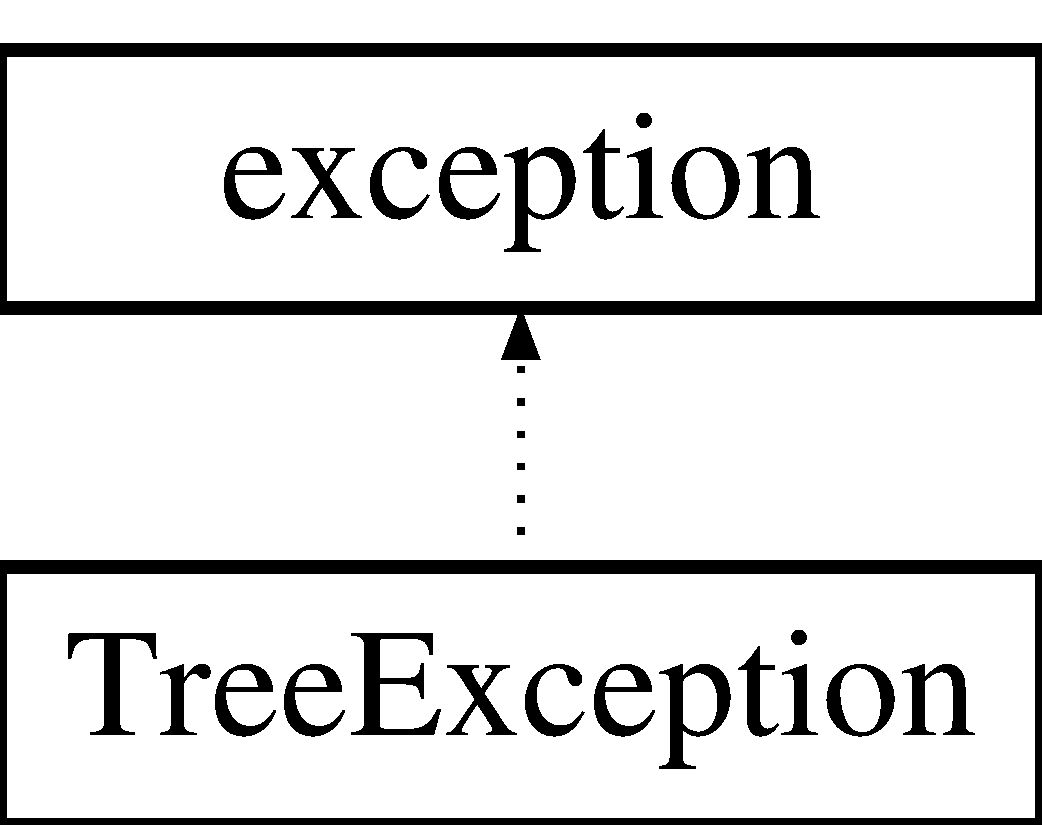
\includegraphics[height=2.000000cm]{class_tree_exception}
\end{center}
\end{figure}
\subsection*{Public Member Functions}
\begin{DoxyCompactItemize}
\item 
\hyperlink{class_tree_exception_aa75b34acf02d0e86fb70a63242894311}{Tree\-Exception} (char $\ast$cause)
\item 
virtual \hyperlink{class_tree_exception_a68dfe698f22aabd8d51b0c533f818263}{$\sim$\-Tree\-Exception} ()  throw ()
\item 
virtual const char $\ast$ \hyperlink{class_tree_exception_ab899a6ec0f82bf770b88ba4982e3d696}{what} () const   throw ()
\end{DoxyCompactItemize}
\subsection*{Private Attributes}
\begin{DoxyCompactItemize}
\item 
char $\ast$ \hyperlink{class_tree_exception_a90175b0c5a1e2a7ebb77cadc92b0388b}{\-\_\-cause}
\end{DoxyCompactItemize}


\subsection{Detailed Description}
exception class for trees 

Usefull to manage errors and the unforeseen 

\subsection{Constructor \& Destructor Documentation}
\hypertarget{class_tree_exception_aa75b34acf02d0e86fb70a63242894311}{\index{Tree\-Exception@{Tree\-Exception}!Tree\-Exception@{Tree\-Exception}}
\index{Tree\-Exception@{Tree\-Exception}!TreeException@{Tree\-Exception}}
\subsubsection[{Tree\-Exception}]{\setlength{\rightskip}{0pt plus 5cm}Tree\-Exception\-::\-Tree\-Exception (
\begin{DoxyParamCaption}
\item[{char $\ast$}]{cause}
\end{DoxyParamCaption}
)}}\label{class_tree_exception_aa75b34acf02d0e86fb70a63242894311}
store exception description constructor called then Tree\-Exceptions are threw 
\begin{DoxyParams}[1]{Parameters}
\mbox{\tt in}  & {\em cause} & description of exception origin \\
\hline
\end{DoxyParams}
\hypertarget{class_tree_exception_a68dfe698f22aabd8d51b0c533f818263}{\index{Tree\-Exception@{Tree\-Exception}!$\sim$\-Tree\-Exception@{$\sim$\-Tree\-Exception}}
\index{$\sim$\-Tree\-Exception@{$\sim$\-Tree\-Exception}!TreeException@{Tree\-Exception}}
\subsubsection[{$\sim$\-Tree\-Exception}]{\setlength{\rightskip}{0pt plus 5cm}virtual Tree\-Exception\-::$\sim$\-Tree\-Exception (
\begin{DoxyParamCaption}
{}
\end{DoxyParamCaption}
) throw  ) \hspace{0.3cm}{\ttfamily [virtual]}}}\label{class_tree_exception_a68dfe698f22aabd8d51b0c533f818263}
destructor currently, do anything special 

\subsection{Member Function Documentation}
\hypertarget{class_tree_exception_ab899a6ec0f82bf770b88ba4982e3d696}{\index{Tree\-Exception@{Tree\-Exception}!what@{what}}
\index{what@{what}!TreeException@{Tree\-Exception}}
\subsubsection[{what}]{\setlength{\rightskip}{0pt plus 5cm}virtual const char$\ast$ Tree\-Exception\-::what (
\begin{DoxyParamCaption}
{}
\end{DoxyParamCaption}
) const throw  ) \hspace{0.3cm}{\ttfamily [virtual]}}}\label{class_tree_exception_ab899a6ec0f82bf770b88ba4982e3d696}
virtual fonction from superclass, usefull to get the exception description 

\subsection{Member Data Documentation}
\hypertarget{class_tree_exception_a90175b0c5a1e2a7ebb77cadc92b0388b}{\index{Tree\-Exception@{Tree\-Exception}!\-\_\-cause@{\-\_\-cause}}
\index{\-\_\-cause@{\-\_\-cause}!TreeException@{Tree\-Exception}}
\subsubsection[{\-\_\-cause}]{\setlength{\rightskip}{0pt plus 5cm}char$\ast$ Tree\-Exception\-::\-\_\-cause\hspace{0.3cm}{\ttfamily [private]}}}\label{class_tree_exception_a90175b0c5a1e2a7ebb77cadc92b0388b}


The documentation for this class was generated from the following file\-:\begin{DoxyCompactItemize}
\item 
src/\hyperlink{tree_8hpp}{tree.\-hpp}\end{DoxyCompactItemize}

\hypertarget{class_tree_string}{\section{Tree\-String Class Reference}
\label{class_tree_string}\index{Tree\-String@{Tree\-String}}
}


\hyperlink{class_tree}{Tree} is a recursive structure using nodes.  




{\ttfamily \#include $<$treestring.\-hpp$>$}

\subsection*{Public Member Functions}
\begin{DoxyCompactItemize}
\item 
\hyperlink{class_tree_string_a13117ec068109c174402c8f60597f243}{Tree\-String} ()
\item 
\hyperlink{class_tree_string_ae522f28db152cfe1376ca74f4d861fa7}{Tree\-String} (const \hyperlink{class_tree_string}{Tree\-String} \&other)
\item 
\hyperlink{class_tree_string_ad4672cc528918926c95098738924f3d2}{$\sim$\-Tree\-String} ()
\item 
int \hyperlink{class_tree_string_ac9ce25eae04196336cd8ac83ec5cb9b6}{height} ()
\item 
void \hyperlink{class_tree_string_ab61ae2b5bdba5d2d7d3a7f170a1d78e5}{put} (const string \&word)
\item 
string \hyperlink{class_tree_string_aed814ffed425fac5893e5a74f641977b}{to\-String} ()
\item 
void \hyperlink{class_tree_string_a51187eb2f3f6ec062a6709ce40b0234f}{get\-Words} (forward\-\_\-list$<$ string $>$ \&list)
\item 
void \hyperlink{class_tree_string_abbea8323b70edd4ac271de19317ac140}{get\-Words\-Frequencies} (forward\-\_\-list$<$ pair$<$ string, int $>$$>$ \&words)
\end{DoxyCompactItemize}
\subsection*{Private Attributes}
\begin{DoxyCompactItemize}
\item 
\hyperlink{class_node}{Node} \hyperlink{class_tree_string_a370851bf8faefb8655a188994715ed31}{\-\_\-root}
\end{DoxyCompactItemize}


\subsection{Detailed Description}
\hyperlink{class_tree}{Tree} is a recursive structure using nodes. 

A root value and subtrees of children, represented as a set of linked nodes. 

\subsection{Constructor \& Destructor Documentation}
\hypertarget{class_tree_string_a13117ec068109c174402c8f60597f243}{\index{Tree\-String@{Tree\-String}!Tree\-String@{Tree\-String}}
\index{Tree\-String@{Tree\-String}!TreeString@{Tree\-String}}
\subsubsection[{Tree\-String}]{\setlength{\rightskip}{0pt plus 5cm}Tree\-String\-::\-Tree\-String (
\begin{DoxyParamCaption}
{}
\end{DoxyParamCaption}
)}}\label{class_tree_string_a13117ec068109c174402c8f60597f243}
First node of the tree Default constructor \hypertarget{class_tree_string_ae522f28db152cfe1376ca74f4d861fa7}{\index{Tree\-String@{Tree\-String}!Tree\-String@{Tree\-String}}
\index{Tree\-String@{Tree\-String}!TreeString@{Tree\-String}}
\subsubsection[{Tree\-String}]{\setlength{\rightskip}{0pt plus 5cm}Tree\-String\-::\-Tree\-String (
\begin{DoxyParamCaption}
\item[{const {\bf Tree\-String} \&}]{other}
\end{DoxyParamCaption}
)}}\label{class_tree_string_ae522f28db152cfe1376ca74f4d861fa7}
Copy constructor \hypertarget{class_tree_string_ad4672cc528918926c95098738924f3d2}{\index{Tree\-String@{Tree\-String}!$\sim$\-Tree\-String@{$\sim$\-Tree\-String}}
\index{$\sim$\-Tree\-String@{$\sim$\-Tree\-String}!TreeString@{Tree\-String}}
\subsubsection[{$\sim$\-Tree\-String}]{\setlength{\rightskip}{0pt plus 5cm}Tree\-String\-::$\sim$\-Tree\-String (
\begin{DoxyParamCaption}
{}
\end{DoxyParamCaption}
)}}\label{class_tree_string_ad4672cc528918926c95098738924f3d2}
Destructor, destroy the whole tree 

\subsection{Member Function Documentation}
\hypertarget{class_tree_string_a51187eb2f3f6ec062a6709ce40b0234f}{\index{Tree\-String@{Tree\-String}!get\-Words@{get\-Words}}
\index{get\-Words@{get\-Words}!TreeString@{Tree\-String}}
\subsubsection[{get\-Words}]{\setlength{\rightskip}{0pt plus 5cm}void Tree\-String\-::get\-Words (
\begin{DoxyParamCaption}
\item[{forward\-\_\-list$<$ string $>$ \&}]{list}
\end{DoxyParamCaption}
)}}\label{class_tree_string_a51187eb2f3f6ec062a6709ce40b0234f}
Put each word in a list The list must be initialized ! 
\begin{DoxyParams}[1]{Parameters}
\mbox{\tt in}  & {\em list} & List containing string for each word stored in \hyperlink{class_tree}{Tree} \\
\hline
\end{DoxyParams}
\hypertarget{class_tree_string_abbea8323b70edd4ac271de19317ac140}{\index{Tree\-String@{Tree\-String}!get\-Words\-Frequencies@{get\-Words\-Frequencies}}
\index{get\-Words\-Frequencies@{get\-Words\-Frequencies}!TreeString@{Tree\-String}}
\subsubsection[{get\-Words\-Frequencies}]{\setlength{\rightskip}{0pt plus 5cm}void Tree\-String\-::get\-Words\-Frequencies (
\begin{DoxyParamCaption}
\item[{forward\-\_\-list$<$ pair$<$ string, int $>$$>$ \&}]{words}
\end{DoxyParamCaption}
)}}\label{class_tree_string_abbea8323b70edd4ac271de19317ac140}
Get a list of all words stored in \hyperlink{class_tree}{Tree} and their frequencies, i.\-e. how times a word was added 
\begin{DoxyParams}{Parameters}
{\em int\mbox{]}} & list List of pair containing for each word in \hyperlink{class_tree}{Tree} his frequency \\
\hline
\end{DoxyParams}
\hypertarget{class_tree_string_ac9ce25eae04196336cd8ac83ec5cb9b6}{\index{Tree\-String@{Tree\-String}!height@{height}}
\index{height@{height}!TreeString@{Tree\-String}}
\subsubsection[{height}]{\setlength{\rightskip}{0pt plus 5cm}int Tree\-String\-::height (
\begin{DoxyParamCaption}
{}
\end{DoxyParamCaption}
)}}\label{class_tree_string_ac9ce25eae04196336cd8ac83ec5cb9b6}
The height of the tree 
\begin{DoxyParams}[1]{Parameters}
\mbox{\tt out}  & {\em hgt} & Height of the tree \\
\hline
\end{DoxyParams}
\hypertarget{class_tree_string_ab61ae2b5bdba5d2d7d3a7f170a1d78e5}{\index{Tree\-String@{Tree\-String}!put@{put}}
\index{put@{put}!TreeString@{Tree\-String}}
\subsubsection[{put}]{\setlength{\rightskip}{0pt plus 5cm}void Tree\-String\-::put (
\begin{DoxyParamCaption}
\item[{const string \&}]{word}
\end{DoxyParamCaption}
)}}\label{class_tree_string_ab61ae2b5bdba5d2d7d3a7f170a1d78e5}
Put a word in the tree 
\begin{DoxyParams}[1]{Parameters}
\mbox{\tt in}  & {\em word} & New element to put into the tree \\
\hline
\end{DoxyParams}
\hypertarget{class_tree_string_aed814ffed425fac5893e5a74f641977b}{\index{Tree\-String@{Tree\-String}!to\-String@{to\-String}}
\index{to\-String@{to\-String}!TreeString@{Tree\-String}}
\subsubsection[{to\-String}]{\setlength{\rightskip}{0pt plus 5cm}string Tree\-String\-::to\-String (
\begin{DoxyParamCaption}
{}
\end{DoxyParamCaption}
)}}\label{class_tree_string_aed814ffed425fac5893e5a74f641977b}
Get a string representation of the \hyperlink{class_tree}{Tree} 
\begin{DoxyParams}[1]{Parameters}
\mbox{\tt out}  & {\em desc} & A string reprensation of the \hyperlink{class_tree}{Tree} where each \hyperlink{class_node}{Node} tag is separated by a comma \\
\hline
\end{DoxyParams}


\subsection{Member Data Documentation}
\hypertarget{class_tree_string_a370851bf8faefb8655a188994715ed31}{\index{Tree\-String@{Tree\-String}!\-\_\-root@{\-\_\-root}}
\index{\-\_\-root@{\-\_\-root}!TreeString@{Tree\-String}}
\subsubsection[{\-\_\-root}]{\setlength{\rightskip}{0pt plus 5cm}{\bf Node} Tree\-String\-::\-\_\-root\hspace{0.3cm}{\ttfamily [private]}}}\label{class_tree_string_a370851bf8faefb8655a188994715ed31}


The documentation for this class was generated from the following file\-:\begin{DoxyCompactItemize}
\item 
src/\hyperlink{treestring_8hpp}{treestring.\-hpp}\end{DoxyCompactItemize}

\hypertarget{class_tree_string_exception}{\section{Tree\-String\-Exception Class Reference}
\label{class_tree_string_exception}\index{Tree\-String\-Exception@{Tree\-String\-Exception}}
}


exception class for trees  




{\ttfamily \#include $<$treestring.\-hpp$>$}

Inheritance diagram for Tree\-String\-Exception\-:\begin{figure}[H]
\begin{center}
\leavevmode
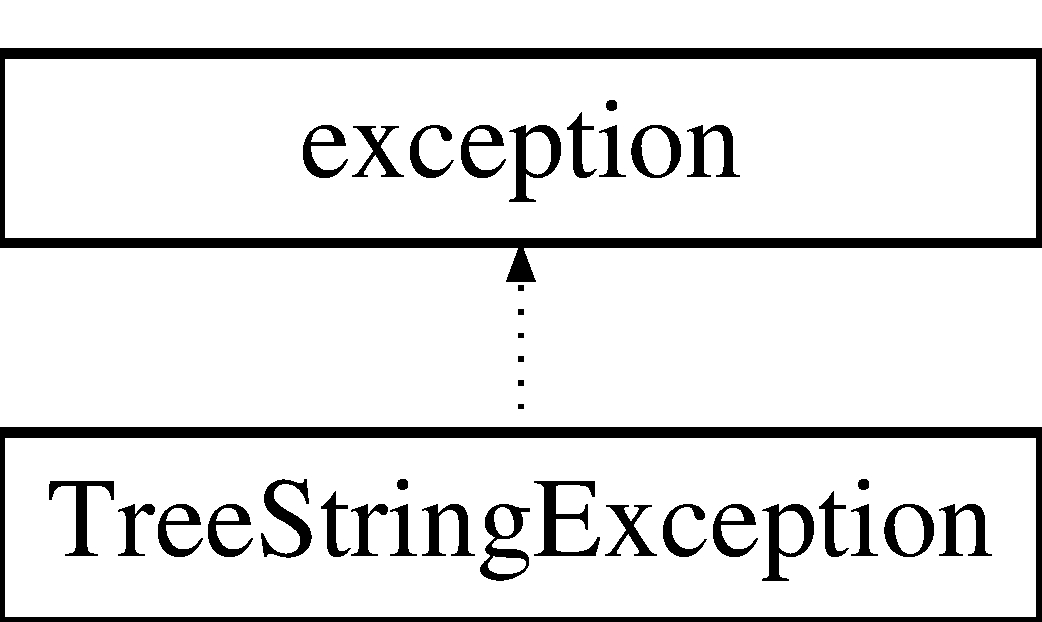
\includegraphics[height=2.000000cm]{class_tree_string_exception}
\end{center}
\end{figure}
\subsection*{Public Member Functions}
\begin{DoxyCompactItemize}
\item 
\hyperlink{class_tree_string_exception_a14c9647a77ce331faddb82724325419a}{Tree\-String\-Exception} (char $\ast$cause)
\item 
virtual \hyperlink{class_tree_string_exception_a4740cacfe385483aa466be7a7399ba82}{$\sim$\-Tree\-String\-Exception} ()  throw ()
\item 
virtual const char $\ast$ \hyperlink{class_tree_string_exception_a80013d6d7031026ea7ab0be964c41713}{what} () const   throw ()
\end{DoxyCompactItemize}
\subsection*{Private Attributes}
\begin{DoxyCompactItemize}
\item 
char $\ast$ \hyperlink{class_tree_string_exception_a4de00ce12f252d1d159211338b999164}{\-\_\-cause}
\end{DoxyCompactItemize}


\subsection{Detailed Description}
exception class for trees 

Usefull to manage errors and the unforeseen 

\subsection{Constructor \& Destructor Documentation}
\hypertarget{class_tree_string_exception_a14c9647a77ce331faddb82724325419a}{\index{Tree\-String\-Exception@{Tree\-String\-Exception}!Tree\-String\-Exception@{Tree\-String\-Exception}}
\index{Tree\-String\-Exception@{Tree\-String\-Exception}!TreeStringException@{Tree\-String\-Exception}}
\subsubsection[{Tree\-String\-Exception}]{\setlength{\rightskip}{0pt plus 5cm}Tree\-String\-Exception\-::\-Tree\-String\-Exception (
\begin{DoxyParamCaption}
\item[{char $\ast$}]{cause}
\end{DoxyParamCaption}
)}}\label{class_tree_string_exception_a14c9647a77ce331faddb82724325419a}
store exception description constructor called then Tree\-Exceptions are threw 
\begin{DoxyParams}[1]{Parameters}
\mbox{\tt in}  & {\em cause} & description of exception origin \\
\hline
\end{DoxyParams}
\hypertarget{class_tree_string_exception_a4740cacfe385483aa466be7a7399ba82}{\index{Tree\-String\-Exception@{Tree\-String\-Exception}!$\sim$\-Tree\-String\-Exception@{$\sim$\-Tree\-String\-Exception}}
\index{$\sim$\-Tree\-String\-Exception@{$\sim$\-Tree\-String\-Exception}!TreeStringException@{Tree\-String\-Exception}}
\subsubsection[{$\sim$\-Tree\-String\-Exception}]{\setlength{\rightskip}{0pt plus 5cm}virtual Tree\-String\-Exception\-::$\sim$\-Tree\-String\-Exception (
\begin{DoxyParamCaption}
{}
\end{DoxyParamCaption}
) throw  ) \hspace{0.3cm}{\ttfamily [virtual]}}}\label{class_tree_string_exception_a4740cacfe385483aa466be7a7399ba82}
destructor currently, do anything special 

\subsection{Member Function Documentation}
\hypertarget{class_tree_string_exception_a80013d6d7031026ea7ab0be964c41713}{\index{Tree\-String\-Exception@{Tree\-String\-Exception}!what@{what}}
\index{what@{what}!TreeStringException@{Tree\-String\-Exception}}
\subsubsection[{what}]{\setlength{\rightskip}{0pt plus 5cm}virtual const char$\ast$ Tree\-String\-Exception\-::what (
\begin{DoxyParamCaption}
{}
\end{DoxyParamCaption}
) const throw  ) \hspace{0.3cm}{\ttfamily [virtual]}}}\label{class_tree_string_exception_a80013d6d7031026ea7ab0be964c41713}
virtual fonction from superclass, usefull to get the exception description 

\subsection{Member Data Documentation}
\hypertarget{class_tree_string_exception_a4de00ce12f252d1d159211338b999164}{\index{Tree\-String\-Exception@{Tree\-String\-Exception}!\-\_\-cause@{\-\_\-cause}}
\index{\-\_\-cause@{\-\_\-cause}!TreeStringException@{Tree\-String\-Exception}}
\subsubsection[{\-\_\-cause}]{\setlength{\rightskip}{0pt plus 5cm}char$\ast$ Tree\-String\-Exception\-::\-\_\-cause\hspace{0.3cm}{\ttfamily [private]}}}\label{class_tree_string_exception_a4de00ce12f252d1d159211338b999164}


The documentation for this class was generated from the following file\-:\begin{DoxyCompactItemize}
\item 
src/\hyperlink{treestring_8hpp}{treestring.\-hpp}\end{DoxyCompactItemize}

\chapter{File Documentation}
\hypertarget{_r_e_a_d_m_e_8md}{\section{\-R\-E\-A\-D\-M\-E.\-md \-File \-Reference}
\label{_r_e_a_d_m_e_8md}\index{\-R\-E\-A\-D\-M\-E.\-md@{\-R\-E\-A\-D\-M\-E.\-md}}
}

\hypertarget{application_8cpp}{\section{src/application.cpp File Reference}
\label{application_8cpp}\index{src/application.\-cpp@{src/application.\-cpp}}
}
{\ttfamily \#include $<$functional$>$}\\*
{\ttfamily \#include $<$iostream$>$}\\*
{\ttfamily \#include $<$fstream$>$}\\*
{\ttfamily \#include \char`\"{}dictionnaire\-\_\-arbre.\-hpp\char`\"{}}\\*
\subsection*{Functions}
\begin{DoxyCompactItemize}
\item 
int \hyperlink{application_8cpp_a217dbf8b442f20279ea00b898af96f52}{main} (int argc, const char $\ast$$\ast$argv)
\end{DoxyCompactItemize}


\subsection{Detailed Description}
\hypertarget{treestring_8hpp_desc}{}\subsection{File description}\label{treestring_8hpp_desc}
Programme permettant de lire des mots dans un fichier texte passé en paramètre et qui calcule leurs fréquence.\hypertarget{treestring_8hpp_copyright}{}\subsection{Copyright}\label{treestring_8hpp_copyright}
This source code is protected by the French intellectual property law.

This program is free software; you can redistribute it and/or modify it under the terms of the G\-N\-U General Public License as published by the Free Software Foundation; version 2 of the License.

This program is distributed in the hope that it will be useful, but W\-I\-T\-H\-O\-U\-T A\-N\-Y W\-A\-R\-R\-A\-N\-T\-Y; without even the implied warranty of M\-E\-R\-C\-H\-A\-N\-T\-A\-B\-I\-L\-I\-T\-Y or F\-I\-T\-N\-E\-S\-S F\-O\-R A P\-A\-R\-T\-I\-C\-U\-L\-A\-R P\-U\-R\-P\-O\-S\-E. See the G\-N\-U General Public License for more details.

You should have received a copy of the G\-N\-U General Public License along with this program; if not, write to the Free Software Foundation, Inc., 51 Franklin Street, Fifth Floor, Boston, M\-A 02110-\/1301, U\-S\-A.\hypertarget{treestring_8hpp_infos}{}\subsection{File informations}\label{treestring_8hpp_infos}
\$\-Date\$ 2014/04/02 \$\-Rev\$ 0.\-2 \$\-Author\$ François Hallereau \& Benjamin Sientzoff \$\-U\-R\-L\$ \href{http://www.github.com/blasterbug/glossygloss}{\tt http\-://www.\-github.\-com/blasterbug/glossygloss} 

\subsection{Function Documentation}
\hypertarget{application_8cpp_a217dbf8b442f20279ea00b898af96f52}{\index{application.\-cpp@{application.\-cpp}!main@{main}}
\index{main@{main}!application.cpp@{application.\-cpp}}
\subsubsection[{main}]{\setlength{\rightskip}{0pt plus 5cm}int main (
\begin{DoxyParamCaption}
\item[{int}]{argc, }
\item[{const char $\ast$$\ast$}]{argv}
\end{DoxyParamCaption}
)}}\label{application_8cpp_a217dbf8b442f20279ea00b898af96f52}

\hypertarget{dictionnaire__arbre_8hpp}{\section{src/dictionnaire\-\_\-arbre.hpp File Reference}
\label{dictionnaire__arbre_8hpp}\index{src/dictionnaire\-\_\-arbre.\-hpp@{src/dictionnaire\-\_\-arbre.\-hpp}}
}
{\ttfamily \#include \char`\"{}treestring.\-hpp\char`\"{}}\\*
{\ttfamily \#include $<$utility$>$}\\*
\subsection*{Classes}
\begin{DoxyCompactItemize}
\item 
class \hyperlink{class_dictionnaire}{Dictionnaire}
\end{DoxyCompactItemize}
\subsection*{Functions}
\begin{DoxyCompactItemize}
\item 
bool \hyperlink{dictionnaire__arbre_8hpp_a7335ea62aecc32d159584bba8bb1fbd2}{tri\-Pair} (const pair$<$ string, int $>$ \&first, const pair$<$ string, int $>$ \&second)
\end{DoxyCompactItemize}


\subsection{Function Documentation}
\hypertarget{dictionnaire__arbre_8hpp_a7335ea62aecc32d159584bba8bb1fbd2}{\index{dictionnaire\-\_\-arbre.\-hpp@{dictionnaire\-\_\-arbre.\-hpp}!tri\-Pair@{tri\-Pair}}
\index{tri\-Pair@{tri\-Pair}!dictionnaire_arbre.hpp@{dictionnaire\-\_\-arbre.\-hpp}}
\subsubsection[{tri\-Pair}]{\setlength{\rightskip}{0pt plus 5cm}bool tri\-Pair (
\begin{DoxyParamCaption}
\item[{const pair$<$ string, int $>$ \&}]{first, }
\item[{const pair$<$ string, int $>$ \&}]{second}
\end{DoxyParamCaption}
)}}\label{dictionnaire__arbre_8hpp_a7335ea62aecc32d159584bba8bb1fbd2}
Fonction qui permet de trier un container de pairs construit avec des strings et des entiers. Le critère de tri est l'ordre naturel sur les entiers appliqué à l'entier de la pair. 
\begin{DoxyParams}[1]{Parameters}
\mbox{\tt in}  & {\em first} & la première pair à comparer \\
\hline
\mbox{\tt in}  & {\em second} & la seconde pair à comparer \\
\hline
\mbox{\tt out}  & {\em bool} & vrai si first$>$seconde sinon faux \\
\hline
\end{DoxyParams}

\hypertarget{dictionnaire__hash_8hpp}{\section{src/dictionnaire\-\_\-hash.hpp File Reference}
\label{dictionnaire__hash_8hpp}\index{src/dictionnaire\-\_\-hash.\-hpp@{src/dictionnaire\-\_\-hash.\-hpp}}
}
{\ttfamily \#include \char`\"{}hashtable.\-hpp\char`\"{}}\\*
{\ttfamily \#include $<$utility$>$}\\*
\subsection*{Classes}
\begin{DoxyCompactItemize}
\item 
class \hyperlink{class_dictionnaire}{Dictionnaire}
\end{DoxyCompactItemize}
\subsection*{Functions}
\begin{DoxyCompactItemize}
\item 
bool \hyperlink{dictionnaire__hash_8hpp_a7335ea62aecc32d159584bba8bb1fbd2}{tri\-Pair} (const pair$<$ string, int $>$ \&first, const pair$<$ string, int $>$ \&second)
\item 
{\footnotesize template$<$$>$ }\\unsigned \hyperlink{dictionnaire__hash_8hpp_a9f9fe4e9cebe86142ae9312c8ea4d458}{computehash$<$ string $>$} (string element)
\end{DoxyCompactItemize}


\subsection{Detailed Description}
\hypertarget{treestring_8hpp_desc}{}\subsection{File description}\label{treestring_8hpp_desc}
\hyperlink{class_dictionnaire}{Dictionnaire} utilisant une \hyperlink{class_hashtable}{Hashtable}\hypertarget{treestring_8hpp_copyright}{}\subsection{Copyright}\label{treestring_8hpp_copyright}
This source code is protected by the French intellectual property law.

This program is free software; you can redistribute it and/or modify it under the terms of the G\-N\-U General Public License as published by the Free Software Foundation; version 2 of the License.

This program is distributed in the hope that it will be useful, but W\-I\-T\-H\-O\-U\-T A\-N\-Y W\-A\-R\-R\-A\-N\-T\-Y; without even the implied warranty of M\-E\-R\-C\-H\-A\-N\-T\-A\-B\-I\-L\-I\-T\-Y or F\-I\-T\-N\-E\-S\-S F\-O\-R A P\-A\-R\-T\-I\-C\-U\-L\-A\-R P\-U\-R\-P\-O\-S\-E. See the G\-N\-U General Public License for more details.

You should have received a copy of the G\-N\-U General Public License along with this program; if not, write to the Free Software Foundation, Inc., 51 Franklin Street, Fifth Floor, Boston, M\-A 02110-\/1301, U\-S\-A.\hypertarget{treestring_8hpp_infos}{}\subsection{File informations}\label{treestring_8hpp_infos}
\$\-Date\$ 2014/03/27 \$\-Rev\$ 0.\-2 \$\-Author\$ Benjamin Sientzoff \& François Hallereau \$\-U\-R\-L\$ \href{http://www.github.com/blasterbug}{\tt http\-://www.\-github.\-com/blasterbug} 

\subsection{Function Documentation}
\hypertarget{dictionnaire__hash_8hpp_a9f9fe4e9cebe86142ae9312c8ea4d458}{\index{dictionnaire\-\_\-hash.\-hpp@{dictionnaire\-\_\-hash.\-hpp}!computehash$<$ string $>$@{computehash$<$ string $>$}}
\index{computehash$<$ string $>$@{computehash$<$ string $>$}!dictionnaire_hash.hpp@{dictionnaire\-\_\-hash.\-hpp}}
\subsubsection[{computehash$<$ string $>$}]{\setlength{\rightskip}{0pt plus 5cm}template$<$$>$ unsigned {\bf computehash}$<$ string $>$ (
\begin{DoxyParamCaption}
\item[{string}]{element}
\end{DoxyParamCaption}
)}}\label{dictionnaire__hash_8hpp_a9f9fe4e9cebe86142ae9312c8ea4d458}
Fonction pour calculer les clés de hashage de string \hypertarget{dictionnaire__hash_8hpp_a7335ea62aecc32d159584bba8bb1fbd2}{\index{dictionnaire\-\_\-hash.\-hpp@{dictionnaire\-\_\-hash.\-hpp}!tri\-Pair@{tri\-Pair}}
\index{tri\-Pair@{tri\-Pair}!dictionnaire_hash.hpp@{dictionnaire\-\_\-hash.\-hpp}}
\subsubsection[{tri\-Pair}]{\setlength{\rightskip}{0pt plus 5cm}bool tri\-Pair (
\begin{DoxyParamCaption}
\item[{const pair$<$ string, int $>$ \&}]{first, }
\item[{const pair$<$ string, int $>$ \&}]{second}
\end{DoxyParamCaption}
)}}\label{dictionnaire__hash_8hpp_a7335ea62aecc32d159584bba8bb1fbd2}
Fonction qui permet de trier un container de pairs construit avec des strings et des entiers. Le critère de tri est l'ordre naturel sur les entiers appliqué à l'entier de la pair. 
\begin{DoxyParams}[1]{Parameters}
\mbox{\tt in}  & {\em first} & la première pair à comparer \\
\hline
\mbox{\tt in}  & {\em second} & la seconde pair à comparer \\
\hline
\mbox{\tt out}  & {\em bool} & vrai si first$>$seconde sinon faux \\
\hline
\end{DoxyParams}

\hypertarget{hashtable_8hpp}{\section{src/hashtable.hpp File Reference}
\label{hashtable_8hpp}\index{src/hashtable.\-hpp@{src/hashtable.\-hpp}}
}
{\ttfamily \#include $<$string$>$}\\*
{\ttfamily \#include $<$cassert$>$}\\*
{\ttfamily \#include $<$utility$>$}\\*
{\ttfamily \#include $<$forward\-\_\-list$>$}\\*
\subsection*{Classes}
\begin{DoxyCompactItemize}
\item 
class \hyperlink{class_hashtable_exception}{Hashtable\-Exception}
\begin{DoxyCompactList}\small\item\em Exception class to manage \hyperlink{class_hashtable}{Hashtable} errors. \end{DoxyCompactList}\item 
class \hyperlink{class_alveole}{Alveole$<$ K, V $>$}
\begin{DoxyCompactList}\small\item\em Class to define \hyperlink{class_hashtable}{Hashtable} alveoles. \end{DoxyCompactList}\item 
class \hyperlink{class_hashtable}{Hashtable$<$ K, V $>$}
\begin{DoxyCompactList}\small\item\em Maps a key to a value. \end{DoxyCompactList}\end{DoxyCompactItemize}
\subsection*{Macros}
\begin{DoxyCompactItemize}
\item 
\#define \hyperlink{hashtable_8hpp_a29fd18bed01c4d836c7ebfe73a125c3f}{E\-N\-D}~nullptr
\begin{DoxyCompactList}\small\item\em macro to define end of alveole chains \end{DoxyCompactList}\item 
\#define \hyperlink{hashtable_8hpp_a78d344caabde729a4559393a0552bf1c}{A\-R\-R\-A\-Y\-S\-I\-Z\-E}~25
\begin{DoxyCompactList}\small\item\em macro to define size of hash arrays \end{DoxyCompactList}\item 
\#define \hyperlink{hashtable_8hpp_a8de3ed741dadc9c979a4ff17c0a9116e}{N\-D\-E\-B\-U\-G}
\end{DoxyCompactItemize}
\subsection*{Functions}
\begin{DoxyCompactItemize}
\item 
{\footnotesize template$<$typename K $>$ }\\unsigned \hyperlink{hashtable_8hpp_a0884e6a3e2395d8a9cec36a7c651820b}{computehash} (\hyperlink{sample__hashtable_8cpp_a97d832ae23af4f215e801e37e4f94254}{K} element)
\end{DoxyCompactItemize}


\subsection{Detailed Description}
\hypertarget{treestring_8hpp_desc}{}\subsection{File description}\label{treestring_8hpp_desc}
data structure to store pairs in a table a hashcode is compute with k to evaluate the suitable place to store the pair

!! W\-A\-R\-N\-I\-N\-G\-: int hash\-Code(\-K key) must be implemented !!\hypertarget{treestring_8hpp_copyright}{}\subsection{Copyright}\label{treestring_8hpp_copyright}
This source code is protected by the French intellectual property law.

This program is free software; you can redistribute it and/or modify it under the terms of the G\-N\-U General Public License as published by the Free Software Foundation; version 2 of the License.

This program is distributed in the hope that it will be useful, but W\-I\-T\-H\-O\-U\-T A\-N\-Y W\-A\-R\-R\-A\-N\-T\-Y; without even the implied warranty of M\-E\-R\-C\-H\-A\-N\-T\-A\-B\-I\-L\-I\-T\-Y or F\-I\-T\-N\-E\-S\-S F\-O\-R A P\-A\-R\-T\-I\-C\-U\-L\-A\-R P\-U\-R\-P\-O\-S\-E. See the G\-N\-U General Public License for more details.

You should have received a copy of the G\-N\-U General Public License along with this program; if not, write to the Free Software Foundation, Inc., 51 Franklin Street, Fifth Floor, Boston, M\-A 02110-\/1301, U\-S\-A.\hypertarget{treestring_8hpp_infos}{}\subsection{File informations}\label{treestring_8hpp_infos}
\$\-Date\$ 2014/03/27 \$\-Rev\$ 0.\-2 \$\-Author\$ Benjamin Sientzoff \$\-U\-R\-L\$ \href{http://www.github.com/blasterbug}{\tt http\-://www.\-github.\-com/blasterbug}

\begin{DoxyRefDesc}{Todo}
\item[\hyperlink{todo__todo000001}{Todo}]\-: removing the last element of a alveoles chain makes trouble (seg fault) \end{DoxyRefDesc}


\subsection{Macro Definition Documentation}
\hypertarget{hashtable_8hpp_a78d344caabde729a4559393a0552bf1c}{\index{hashtable.\-hpp@{hashtable.\-hpp}!A\-R\-R\-A\-Y\-S\-I\-Z\-E@{A\-R\-R\-A\-Y\-S\-I\-Z\-E}}
\index{A\-R\-R\-A\-Y\-S\-I\-Z\-E@{A\-R\-R\-A\-Y\-S\-I\-Z\-E}!hashtable.hpp@{hashtable.\-hpp}}
\subsubsection[{A\-R\-R\-A\-Y\-S\-I\-Z\-E}]{\setlength{\rightskip}{0pt plus 5cm}\#define A\-R\-R\-A\-Y\-S\-I\-Z\-E~25}}\label{hashtable_8hpp_a78d344caabde729a4559393a0552bf1c}


macro to define size of hash arrays 

\hypertarget{hashtable_8hpp_a29fd18bed01c4d836c7ebfe73a125c3f}{\index{hashtable.\-hpp@{hashtable.\-hpp}!E\-N\-D@{E\-N\-D}}
\index{E\-N\-D@{E\-N\-D}!hashtable.hpp@{hashtable.\-hpp}}
\subsubsection[{E\-N\-D}]{\setlength{\rightskip}{0pt plus 5cm}\#define E\-N\-D~nullptr}}\label{hashtable_8hpp_a29fd18bed01c4d836c7ebfe73a125c3f}


macro to define end of alveole chains 

\hypertarget{hashtable_8hpp_a8de3ed741dadc9c979a4ff17c0a9116e}{\index{hashtable.\-hpp@{hashtable.\-hpp}!N\-D\-E\-B\-U\-G@{N\-D\-E\-B\-U\-G}}
\index{N\-D\-E\-B\-U\-G@{N\-D\-E\-B\-U\-G}!hashtable.hpp@{hashtable.\-hpp}}
\subsubsection[{N\-D\-E\-B\-U\-G}]{\setlength{\rightskip}{0pt plus 5cm}\#define N\-D\-E\-B\-U\-G}}\label{hashtable_8hpp_a8de3ed741dadc9c979a4ff17c0a9116e}


\subsection{Function Documentation}
\hypertarget{hashtable_8hpp_a0884e6a3e2395d8a9cec36a7c651820b}{\index{hashtable.\-hpp@{hashtable.\-hpp}!computehash@{computehash}}
\index{computehash@{computehash}!hashtable.hpp@{hashtable.\-hpp}}
\subsubsection[{computehash}]{\setlength{\rightskip}{0pt plus 5cm}template$<$typename K $>$ unsigned computehash (
\begin{DoxyParamCaption}
\item[{{\bf K}}]{element}
\end{DoxyParamCaption}
)}}\label{hashtable_8hpp_a0884e6a3e2395d8a9cec36a7c651820b}
Fonction you must define when you're using Hashable An exemple is given in the sample file 
\begin{DoxyParams}[1]{Parameters}
\mbox{\tt in}  & {\em element} & element to compute hashcode from \\
\hline
\mbox{\tt out}  & {\em hashcode} & the hashcode of element, an unsigned integer\\
\hline
\end{DoxyParams}
template$<$$>$ unisgned \hyperlink{dictionnaire__hash_8hpp_a9f9fe4e9cebe86142ae9312c8ea4d458}{computehash$<$string$>$(string element)}

your implementation of hashcode function 
\hypertarget{sample__hashtable_8cpp}{\section{src/sample\-\_\-hashtable.cpp File Reference}
\label{sample__hashtable_8cpp}\index{src/sample\-\_\-hashtable.\-cpp@{src/sample\-\_\-hashtable.\-cpp}}
}
{\ttfamily \#include $<$functional$>$}\\*
{\ttfamily \#include $<$iostream$>$}\\*
{\ttfamily \#include $<$cstdlib$>$}\\*
{\ttfamily \#include $<$fstream$>$}\\*
{\ttfamily \#include \char`\"{}hashtable.\-hpp\char`\"{}}\\*
\subsection*{Macros}
\begin{DoxyCompactItemize}
\item 
\#define \hyperlink{sample__hashtable_8cpp_a97d832ae23af4f215e801e37e4f94254}{K}~string
\item 
\#define \hyperlink{sample__hashtable_8cpp_af40a326b23c68a27cebe60f16634a2cb}{V}~string
\end{DoxyCompactItemize}
\subsection*{Functions}
\begin{DoxyCompactItemize}
\item 
{\footnotesize template$<$$>$ }\\unsigned \hyperlink{sample__hashtable_8cpp_ae31ffa0e4fbbbcb53f4e30048ba55b66}{computehash$<$ K $>$} (\hyperlink{sample__hashtable_8cpp_a97d832ae23af4f215e801e37e4f94254}{K} element)
\item 
int \hyperlink{sample__hashtable_8cpp_a217dbf8b442f20279ea00b898af96f52}{main} (int argc, const char $\ast$$\ast$argv)
\end{DoxyCompactItemize}


\subsection{Detailed Description}
\hypertarget{treestring_8hpp_desc}{}\subsection{File description}\label{treestring_8hpp_desc}
a sample of hashtable usages.\hypertarget{treestring_8hpp_copyright}{}\subsection{Copyright}\label{treestring_8hpp_copyright}
This source code is protected by the French intellectual property law.

This program is free software; you can redistribute it and/or modify it under the terms of the G\-N\-U General Public License as published by the Free Software Foundation; version 2 of the License.

This program is distributed in the hope that it will be useful, but W\-I\-T\-H\-O\-U\-T A\-N\-Y W\-A\-R\-R\-A\-N\-T\-Y; without even the implied warranty of M\-E\-R\-C\-H\-A\-N\-T\-A\-B\-I\-L\-I\-T\-Y or F\-I\-T\-N\-E\-S\-S F\-O\-R A P\-A\-R\-T\-I\-C\-U\-L\-A\-R P\-U\-R\-P\-O\-S\-E. See the G\-N\-U General Public License for more details.

You should have received a copy of the G\-N\-U General Public License along with this program; if not, write to the Free Software Foundation, Inc., 51 Franklin Street, Fifth Floor, Boston, M\-A 02110-\/1301, U\-S\-A.\hypertarget{treestring_8hpp_infos}{}\subsection{File informations}\label{treestring_8hpp_infos}
\$\-Date\$ 2014/03/28 \$\-Rev\$ 0.\-1 \$\-Author\$ Benjamin Sientzoff \$\-U\-R\-L\$ \href{http://www.github.com/blasterbug}{\tt http\-://www.\-github.\-com/blasterbug} 

\subsection{Macro Definition Documentation}
\hypertarget{sample__hashtable_8cpp_a97d832ae23af4f215e801e37e4f94254}{\index{sample\-\_\-hashtable.\-cpp@{sample\-\_\-hashtable.\-cpp}!K@{K}}
\index{K@{K}!sample_hashtable.cpp@{sample\-\_\-hashtable.\-cpp}}
\subsubsection[{K}]{\setlength{\rightskip}{0pt plus 5cm}\#define K~string}}\label{sample__hashtable_8cpp_a97d832ae23af4f215e801e37e4f94254}
\hypertarget{sample__hashtable_8cpp_af40a326b23c68a27cebe60f16634a2cb}{\index{sample\-\_\-hashtable.\-cpp@{sample\-\_\-hashtable.\-cpp}!V@{V}}
\index{V@{V}!sample_hashtable.cpp@{sample\-\_\-hashtable.\-cpp}}
\subsubsection[{V}]{\setlength{\rightskip}{0pt plus 5cm}\#define V~string}}\label{sample__hashtable_8cpp_af40a326b23c68a27cebe60f16634a2cb}


\subsection{Function Documentation}
\hypertarget{sample__hashtable_8cpp_ae31ffa0e4fbbbcb53f4e30048ba55b66}{\index{sample\-\_\-hashtable.\-cpp@{sample\-\_\-hashtable.\-cpp}!computehash$<$ K $>$@{computehash$<$ K $>$}}
\index{computehash$<$ K $>$@{computehash$<$ K $>$}!sample_hashtable.cpp@{sample\-\_\-hashtable.\-cpp}}
\subsubsection[{computehash$<$ K $>$}]{\setlength{\rightskip}{0pt plus 5cm}template$<$$>$ unsigned {\bf computehash}$<$ {\bf K} $>$ (
\begin{DoxyParamCaption}
\item[{{\bf K}}]{element}
\end{DoxyParamCaption}
)}}\label{sample__hashtable_8cpp_ae31ffa0e4fbbbcb53f4e30048ba55b66}
\hypertarget{sample__hashtable_8cpp_a217dbf8b442f20279ea00b898af96f52}{\index{sample\-\_\-hashtable.\-cpp@{sample\-\_\-hashtable.\-cpp}!main@{main}}
\index{main@{main}!sample_hashtable.cpp@{sample\-\_\-hashtable.\-cpp}}
\subsubsection[{main}]{\setlength{\rightskip}{0pt plus 5cm}int main (
\begin{DoxyParamCaption}
\item[{int}]{argc, }
\item[{const char $\ast$$\ast$}]{argv}
\end{DoxyParamCaption}
)}}\label{sample__hashtable_8cpp_a217dbf8b442f20279ea00b898af96f52}

\hypertarget{sample__tree_8cpp}{\section{src/sample\-\_\-tree.cpp File Reference}
\label{sample__tree_8cpp}\index{src/sample\-\_\-tree.\-cpp@{src/sample\-\_\-tree.\-cpp}}
}
{\ttfamily \#include $<$functional$>$}\\*
{\ttfamily \#include $<$iostream$>$}\\*
{\ttfamily \#include $<$cstdlib$>$}\\*
{\ttfamily \#include $<$fstream$>$}\\*
{\ttfamily \#include \char`\"{}tree.\-hpp\char`\"{}}\\*
\subsection*{Functions}
\begin{DoxyCompactItemize}
\item 
int \hyperlink{sample__tree_8cpp_a217dbf8b442f20279ea00b898af96f52}{main} (int argc, const char $\ast$$\ast$argv)
\end{DoxyCompactItemize}


\subsection{Detailed Description}
\hypertarget{treestring_8hpp_desc}{}\subsection{File description}\label{treestring_8hpp_desc}
a sample showing how to use a \hyperlink{class_tree}{Tree}\hypertarget{treestring_8hpp_copyright}{}\subsection{Copyright}\label{treestring_8hpp_copyright}
This source code is protected by the French intellectual property law.

This program is free software; you can redistribute it and/or modify it under the terms of the G\-N\-U General Public License as published by the Free Software Foundation; version 2 of the License.

This program is distributed in the hope that it will be useful, but W\-I\-T\-H\-O\-U\-T A\-N\-Y W\-A\-R\-R\-A\-N\-T\-Y; without even the implied warranty of M\-E\-R\-C\-H\-A\-N\-T\-A\-B\-I\-L\-I\-T\-Y or F\-I\-T\-N\-E\-S\-S F\-O\-R A P\-A\-R\-T\-I\-C\-U\-L\-A\-R P\-U\-R\-P\-O\-S\-E. See the G\-N\-U General Public License for more details.

You should have received a copy of the G\-N\-U General Public License along with this program; if not, write to the Free Software Foundation, Inc., 51 Franklin Street, Fifth Floor, Boston, M\-A 02110-\/1301, U\-S\-A.\hypertarget{treestring_8hpp_infos}{}\subsection{File informations}\label{treestring_8hpp_infos}
\$\-Date\$ 2014/04/03 \$\-Rev\$ 0.\-1 \$\-Author\$ Benjamin Sientzoff \$\-U\-R\-L\$ \href{http://www.github.com/blasterbug}{\tt http\-://www.\-github.\-com/blasterbug} 

\subsection{Function Documentation}
\hypertarget{sample__tree_8cpp_a217dbf8b442f20279ea00b898af96f52}{\index{sample\-\_\-tree.\-cpp@{sample\-\_\-tree.\-cpp}!main@{main}}
\index{main@{main}!sample_tree.cpp@{sample\-\_\-tree.\-cpp}}
\subsubsection[{main}]{\setlength{\rightskip}{0pt plus 5cm}int main (
\begin{DoxyParamCaption}
\item[{int}]{argc, }
\item[{const char $\ast$$\ast$}]{argv}
\end{DoxyParamCaption}
)}}\label{sample__tree_8cpp_a217dbf8b442f20279ea00b898af96f52}

\hypertarget{sample__treestring_8cpp}{\section{src/sample\-\_\-treestring.cpp File Reference}
\label{sample__treestring_8cpp}\index{src/sample\-\_\-treestring.\-cpp@{src/sample\-\_\-treestring.\-cpp}}
}
{\ttfamily \#include $<$functional$>$}\\*
{\ttfamily \#include $<$iostream$>$}\\*
{\ttfamily \#include $<$cstdlib$>$}\\*
{\ttfamily \#include $<$fstream$>$}\\*
{\ttfamily \#include \char`\"{}treestring.\-hpp\char`\"{}}\\*
\subsection*{Functions}
\begin{DoxyCompactItemize}
\item 
int \hyperlink{sample__treestring_8cpp_a217dbf8b442f20279ea00b898af96f52}{main} (int argc, const char $\ast$$\ast$argv)
\end{DoxyCompactItemize}


\subsection{Detailed Description}
\hypertarget{treestring_8hpp_desc}{}\subsection{File description}\label{treestring_8hpp_desc}
a sample to show how to use \hyperlink{class_tree_string}{Tree\-String} class\hypertarget{treestring_8hpp_copyright}{}\subsection{Copyright}\label{treestring_8hpp_copyright}
This source code is protected by the French intellectual property law.

This program is free software; you can redistribute it and/or modify it under the terms of the G\-N\-U General Public License as published by the Free Software Foundation; version 2 of the License.

This program is distributed in the hope that it will be useful, but W\-I\-T\-H\-O\-U\-T A\-N\-Y W\-A\-R\-R\-A\-N\-T\-Y; without even the implied warranty of M\-E\-R\-C\-H\-A\-N\-T\-A\-B\-I\-L\-I\-T\-Y or F\-I\-T\-N\-E\-S\-S F\-O\-R A P\-A\-R\-T\-I\-C\-U\-L\-A\-R P\-U\-R\-P\-O\-S\-E. See the G\-N\-U General Public License for more details.

You should have received a copy of the G\-N\-U General Public License along with this program; if not, write to the Free Software Foundation, Inc., 51 Franklin Street, Fifth Floor, Boston, M\-A 02110-\/1301, U\-S\-A.\hypertarget{treestring_8hpp_infos}{}\subsection{File informations}\label{treestring_8hpp_infos}
\$\-Date\$ 2014/04/21 \$\-Rev\$ 0.\-1 \$\-Author\$ Benjamin Sientzoff \$\-U\-R\-L\$ \href{http://www.github.com/blasterbug}{\tt http\-://www.\-github.\-com/blasterbug} 

\subsection{Function Documentation}
\hypertarget{sample__treestring_8cpp_a217dbf8b442f20279ea00b898af96f52}{\index{sample\-\_\-treestring.\-cpp@{sample\-\_\-treestring.\-cpp}!main@{main}}
\index{main@{main}!sample_treestring.cpp@{sample\-\_\-treestring.\-cpp}}
\subsubsection[{main}]{\setlength{\rightskip}{0pt plus 5cm}int main (
\begin{DoxyParamCaption}
\item[{int}]{argc, }
\item[{const char $\ast$$\ast$}]{argv}
\end{DoxyParamCaption}
)}}\label{sample__treestring_8cpp_a217dbf8b442f20279ea00b898af96f52}

\hypertarget{tree_8hpp}{\section{src/tree.hpp File Reference}
\label{tree_8hpp}\index{src/tree.\-hpp@{src/tree.\-hpp}}
}
{\ttfamily \#include $<$string$>$}\\*
{\ttfamily \#include $<$forward\-\_\-list$>$}\\*
\subsection*{Classes}
\begin{DoxyCompactItemize}
\item 
class \hyperlink{class_tree_exception}{Tree\-Exception}
\begin{DoxyCompactList}\small\item\em exception class for trees \end{DoxyCompactList}\item 
class \hyperlink{class_node}{Node$<$ T $>$}
\begin{DoxyCompactList}\small\item\em Defines tree nodes. \end{DoxyCompactList}\item 
class \hyperlink{class_tree}{Tree$<$ T $>$}
\begin{DoxyCompactList}\small\item\em \hyperlink{class_tree}{Tree} is a recursive structure using nodes. \end{DoxyCompactList}\end{DoxyCompactItemize}


\subsection{Detailed Description}
\hypertarget{treestring_8hpp_desc}{}\subsection{File description}\label{treestring_8hpp_desc}
\hyperlink{class_tree}{Tree} is a recursive structure using nodes. \hyperlink{class_node}{Node} stores a value (tag) and has several children\hypertarget{treestring_8hpp_copyright}{}\subsection{Copyright}\label{treestring_8hpp_copyright}
This source code is protected by the French intellectual property law.

This program is free software; you can redistribute it and/or modify it under the terms of the G\-N\-U General Public License as published by the Free Software Foundation; version 2 of the License.

This program is distributed in the hope that it will be useful, but W\-I\-T\-H\-O\-U\-T A\-N\-Y W\-A\-R\-R\-A\-N\-T\-Y; without even the implied warranty of M\-E\-R\-C\-H\-A\-N\-T\-A\-B\-I\-L\-I\-T\-Y or F\-I\-T\-N\-E\-S\-S F\-O\-R A P\-A\-R\-T\-I\-C\-U\-L\-A\-R P\-U\-R\-P\-O\-S\-E. See the G\-N\-U General Public License for more details.

You should have received a copy of the G\-N\-U General Public License along with this program; if not, write to the Free Software Foundation, Inc., 51 Franklin Street, Fifth Floor, Boston, M\-A 02110-\/1301, U\-S\-A.\hypertarget{treestring_8hpp_infos}{}\subsection{File informations}\label{treestring_8hpp_infos}
\$\-Date\$ 2014/03/27 \$\-Rev\$ 0.\-3 \$\-Author\$ Benjamin Sientzoff \$\-U\-R\-L\$ \href{http://www.github.com/blasterbug}{\tt http\-://www.\-github.\-com/blasterbug} 
\hypertarget{treestring_8hpp}{\section{src/treestring.hpp File Reference}
\label{treestring_8hpp}\index{src/treestring.\-hpp@{src/treestring.\-hpp}}
}
{\ttfamily \#include $<$cassert$>$}\\*
{\ttfamily \#include $<$string$>$}\\*
{\ttfamily \#include $<$forward\-\_\-list$>$}\\*
{\ttfamily \#include $<$utility$>$}\\*
{\ttfamily \#include $<$sstream$>$}\\*
\subsection*{Classes}
\begin{DoxyCompactItemize}
\item 
class \hyperlink{class_tree_string_exception}{Tree\-String\-Exception}
\begin{DoxyCompactList}\small\item\em exception class for trees \end{DoxyCompactList}\item 
class \hyperlink{class_node}{Node$<$ T $>$}
\begin{DoxyCompactList}\small\item\em Defines tree nodes. \end{DoxyCompactList}\item 
class \hyperlink{class_tree_string}{Tree\-String}
\begin{DoxyCompactList}\small\item\em \hyperlink{class_tree}{Tree} is a recursive structure using nodes. \end{DoxyCompactList}\end{DoxyCompactItemize}


\subsection{Detailed Description}
\hypertarget{treestring_8hpp_desc}{}\subsection{File description}\label{treestring_8hpp_desc}
\hyperlink{class_tree_string}{Tree\-String} is a recursive structure using nodes. a \hyperlink{class_node}{Node} stores a letter and has several children\hypertarget{treestring_8hpp_copyright}{}\subsection{Copyright}\label{treestring_8hpp_copyright}
This source code is protected by the French intellectual property law.

This program is free software; you can redistribute it and/or modify it under the terms of the G\-N\-U General Public License as published by the Free Software Foundation; version 2 of the License.

This program is distributed in the hope that it will be useful, but W\-I\-T\-H\-O\-U\-T A\-N\-Y W\-A\-R\-R\-A\-N\-T\-Y; without even the implied warranty of M\-E\-R\-C\-H\-A\-N\-T\-A\-B\-I\-L\-I\-T\-Y or F\-I\-T\-N\-E\-S\-S F\-O\-R A P\-A\-R\-T\-I\-C\-U\-L\-A\-R P\-U\-R\-P\-O\-S\-E. See the G\-N\-U General Public License for more details.

You should have received a copy of the G\-N\-U General Public License along with this program; if not, write to the Free Software Foundation, Inc., 51 Franklin Street, Fifth Floor, Boston, M\-A 02110-\/1301, U\-S\-A.\hypertarget{treestring_8hpp_infos}{}\subsection{File informations}\label{treestring_8hpp_infos}
\$\-Date\$ 2014/04/5 \$\-Rev\$ 0.\-1 \$\-Author\$ Benjamin Sientzoff \$\-U\-R\-L\$ \href{http://www.github.com/blasterbug}{\tt http\-://www.\-github.\-com/blasterbug} 
%--- End generated contents ---

% Index
\newpage
\phantomsection
\addcontentsline{toc}{chapter}{Index}
\printindex

\end{document}
